% Template for a Computer Science Tripos Part II project dissertation
\documentclass[12pt,a4paper,twoside,openright]{report}
\usepackage[pdfborder={0 0 0}]{hyperref}    % turns references into hyperlinks
\usepackage[margin=25mm]{geometry}  % adjusts page layout
\usepackage{graphicx}  % allows inclusion of PDF, PNG and JPG images
\usepackage{verbatim}
\usepackage{docmute}   % only needed to allow inclusion of proposal.tex
\usepackage{tikz}
\usetikzlibrary{shapes.geometric, arrows}
\usepackage{multirow}
\usepackage{url}
\usepackage{csquotes}
\usepackage{float}
\usepackage{textcomp}
 

\raggedbottom                           % try to avoid widows and orphans
\sloppy
\clubpenalty1000%
\widowpenalty1000%

\renewcommand{\baselinestretch}{1.1}    % adjust line spacing to make
                                        % more readable

\begin{document}

\bibliographystyle{plain}


%%%%%%%%%%%%%%%%%%%%%%%%%%%%%%%%%%%%%%%%%%%%%%%%%%%%%%%%%%%%%%%%%%%%%%%%
% Title


\pagestyle{empty}

\rightline{\LARGE \textbf{Simonas Mulevicius}}

\vspace*{60mm}
\begin{center}
\Huge
\textbf{QUIC offloading using NetFPGA smart NICs} \\[5mm]
Computer Science Tripos -- Part II \\[5mm]
Homerton College \\[5mm]
\today  % today's date
\end{center}

%%%%%%%%%%%%%%%%%%%%%%%%%%%%%%%%%%%%%%%%%%%%%%%%%%%%%%%%%%%%%%%%%%%%%%%%%%%%%%
% Proforma, table of contents and list of figures

\pagestyle{plain}

\chapter*{Proforma}

{\large
\begin{tabular}{ll}
Name:               & \bf Simonas Mulevicius                       \\
College:            & \bf Homerton College                     \\
Project Title:      & \bf QUIC offloading using NetFPGA smart NICs \\
Examination:        & \bf Computer Science Tripos -- Part II, July 2021  \\
Word Count:         & \bf 3706\footnotemark[1] \\
Project Originator: & Dr Andrew W. Moore                \\
Supervisor:         & Dr Andrew W. Moore                \\ 
\end{tabular}
}
\footnotetext[1]{This word count was computed
by \texttt{DISS\_LENGTH=\$(detex diss.tex | tr -cd '0-9A-Za-z $\tt\backslash$n' | wc -w); PROPOSAL\_LENGTH=\$(detex proposal.tex | tr -cd '0-9A-Za-z $\tt\backslash$n' | wc -w); echo "\$((\$DISS\_LENGTH-\$PROPOSAL\_LENGTH))"}}

\stepcounter{footnote}


\section*{Original Aims of the Project}

TODO

\section*{Work Completed}

TODO

\section*{Special Difficulties}

For this project, I used two dedicated experimental machines for network testing. 
However, I had accessibility issues during the winter vacation when I was abroad at home.
In particular, I spent more than one month working on the remote set-up, but I could not configure two additional backup machines in the Computer Laboratory.
A suspected issue is a possible hardware fault.
Hence, to continue working on the project, I had to return to my college room, where I had physical access to another pair of specialised computers.
 
 
 
\newpage










\section*{Declaration}

I, Simonas Mulevicius of Homerton College, being a candidate for Part II of the Computer
Science Tripos, hereby declare
that this dissertation and the work described in it are my own work,
unaided except as may be specified below, and that the dissertation
does not contain material that has already been used to any substantial
extent for a comparable purpose. I am content for my dissertation to
be made available to the students and staff of the University.

\bigskip
\leftline{Signed [signature]}

\medskip
\leftline{Date [date]}







%Professional Practice and Presentation 14%
%Introduction and Preparation 26%
%Implementation 40%
%Evaluation and Conclusion 20%




\tableofcontents

\listoffigures

\newpage
\section*{Acknowledgements}

The following people helped with the project setup or provided useful insights or hints on how to tackle project-related problems:
\begin{itemize}
    \item \textbf{Dr Marcin Wojcik} helped with general inquiries related to the setup of NetFPGA developing platform;
    \item \textbf{Professor Andrew W. Moore} was my project supervisor and originator of the project idea;
    \item \textbf{Dr Malcolm Scott} helped with the configuration of two remote backup machines in the Computer Laboratory during the winter vacation;
    \item \textbf{Mr Tatsuhiro Tsujikawa} is the author of \texttt{ngtcp2}\footnote{specific implementation of QUIC which is used in this project}, and he answered usability questions related to it. Moreover, he provided guidance on how null encryption could be turned on in \texttt{ngtcp2};
    \item Part II students \textbf{Ms Akvile Valentukonyte} and \textbf{Mr Justas Janickas} participated in our weekly meetings where we all shared our achieved progress;
\end{itemize}

Furthermore, this document is written using a default dissertation template provided by Martin Richards \cite{how_to_write_a_dissertation_in_LATEX}.
However, some formatting ideas are taken from Alex Coplan's dissertation \cite{Alex_Coplan_dissertation}, which, according to \cite{Computer_Lab_dissertations}, is \enquote{highly commended by the examiners}.

%%%%%%%%%%%%%%%%%%%%%%%%%%%%%%%%%%%%%%%%%%%%%%%%%%%%%%%%%%%%%%%%%%%%%%%
% now for the chapters

\pagestyle{headings}

\chapter{Introduction}
In this chapter, I briefly introduce \texttt{QUIC}, then I give the project's motivation, and I finish the chapter with an overview of \texttt{QUIC} performance measurements performed by other scientists.

% ------------------------------------------------
% TODO
%
% The introduction should explain the principal motivation for the project and show how the work fits into the broad area of surrounding computer science and give a brief survey of previous related work. It should generally be unnecessary to quote at length from technical papers or textbooks. If a simple bibliographic reference is insufficient, consign any lengthy quotation to an appendix.



% FROM: https://www.cst.cam.ac.uk/teaching/part-ii/projects/assessment
% Clear motivation, justifying potential benefits of success.
%Good or excellent requirements analysis; justified and documented selection of suitable tools; good engineering approach.
%Clear presentation of challenging background material covering a range of computer science topics beyond Part IB.
% ------------------------------------------------



% TODO: say what the problem is
% > explain the problem
% > why is the problem interesting?
% > why does the solution enable?

% TODO: describe my work
% > how does my work solve the problem (high-level overview)?
% > details in other chapters


\section{Motivation of the project}
% TODO add reference to the ideas of this paragraph:
Nowadays, more and more people have access to the Internet.
As the scale of the web continues to grow, both companies and researchers look for ways to satisfy ever-increasing market demand to improve the user experience of Internet users.
Customers expect cheap, high-throughput and low latency Internet connection.
However, in the last decade, several trends have emerged.
For example, in recent years, we observed a proliferation of mobile devices - according to \cite{bib_number_of_mobile_users}, at the time of writing, around $92.6\%$ of Internet users used mobile devices to connect to the Internet.
Furthermore, we see the changing patterns of web development.
In particular, usual websites nowadays contain multiple embedded objects of various sizes (e.g. from \texttt{JavaScript} or \texttt{CSS} files to numerous images and videos)\cite{bib_Netdev_0x13_QUIC_Tutorial}.
But, these websites look entirely different from the simple, single document \texttt{HTML} websites used in the early days of the Internet.
% TODO [NOT MY IDEA! -> add source]
Hence, the changing constraints and networking trends encourage us to re-evaluate past protocols.
By using innovative solutions, we can continue improving the performance of the Internet. 
One of such ideas is \texttt{QUIC} - the new transport layer protocol.



This project tries to understand the bottlenecks of \texttt{QUIC} and its performance behaviour.
\texttt{QUIC} transport layer protocol is still in the early development stage.
However, we already need to start thinking about its performance.
Otherwise, there is a possibility that because of the low QUIC throughput, it may not be widely adopted (as happened with earlier attempts to improve \texttt{TCP}). 
% TODO: add a reference to the source proving this claim


The introduction of \texttt{QUIC} would be especially beneficial for countries that do not have access to the low latency Internet connection.
% TODO: give a reason why and add a reference to the author of this idea 
The most interesting part of this project is that  \texttt{QUIC} is a relatively new network technology and, as far as I am aware, there have not been any similar projects which tried to measure \texttt{QUIC}’s performance by \enquote{breaking} it (i.e. using \texttt{QUIC} without encryption).

This analysis could be useful in the future when \texttt{QUIC}’s cryptographic operations would be offloaded to hardware. Nevertheless, these experiments could also have some tangible value for current times. 
For instance, an experimental \texttt{QUIC} with null encryption could be used in secure networks controlled by a single entity (e.g. within a data centre).



%-------IDEAS to add to this section:-------


%The performance study of QUIC under several variable conditions (e.g. packet loss, reordering and delay) in comparison with iperf is the focus of my work.
 
 
%The purpose of this work is to predict future bottlenecks. To achieve this, I would first need to exclude/bypass the cryptographic operations of  \texttt{QUIC}. I already have the functionality to turn on null-encryption on the server-side, so I would need to adopt similar ideas for the  \texttt{QUIC} client. Such a set-up would simulate offloaded encryption. Previous studies analysed different implementations of  \texttt{QUIC} (not ngtcp2), so the primary goal would be to run similar experiments with ngtcp2. After that, I would have to identify situations where  \texttt{QUIC} (ngtcp2 in particular) outperforms TCP using different network conditions. To achieve this, I have a complete testing environment with a configured intermediate machine that can introduce traffic perturbations. In addition, I have already performed some performance measurements using different MTUs. Furthermore, I estimated the impact of core pinning for these tests and took into account both hyperthreading and GSO.
 
 

\subsection{High-Level Overview of \texttt{QUIC}}
I delve into more detail about \texttt{QUIC} in the later sections of the dissertation (see section~\ref{QUIC_details_section}) but briefly speaking \texttt{QUIC} is a new transport layer protocol that combines ideas of \texttt{TCP}, \texttt{HTTP} and other experimental protocols such as \texttt{SPDY} (which is also described in the later sections - see \ref{Previous_attempt_to_improve_http_by_using_SPDY_and_HTTP2}).
On the one hand, \texttt{QUIC} breaks the separation of transport and security layer protocols. 
On the other hand, \texttt{QUIC} protocol offers some performance benefits for modern-day traffic flows (see section~\ref{QUIC_advantages}).


\subsection{Why are performance measurements of \texttt{QUIC} important?}

\texttt{QUIC}, after being publicly launched by \texttt{Google} in 2013 \cite{Chromium_Blog_Experimenting_with_quic}, \texttt{QUIC} is still a relatively new protocol that is still in the development stage.
Hence, any performance measurements of \texttt{QUIC} could guide the ongoing efforts to build this new high-performance transport layer protocol.
Furthermore, there are strong indications showing that \texttt{QUIC} could be widely adopted in the future.
For instance, \texttt{Google}, one of the major advocates for \texttt{QUIC}, operates both on the server side (e.g. search engine or video streaming service \texttt{YouTube}) and the client side (e.g. \texttt{Google Chrome} browser for desktop and mobile devices) \cite{A_QUICk_Introduction_to_HTTP3}.
Hence, using its existing market presence \texttt{Google} could potentially encourage the faster adoption of \texttt{QUIC}.
Actually, according to the report published in 2016\cite{RuthJan2018AFLa}, at that time around 40\% of all traffic of \texttt{Google} was using \texttt{QUIC}.
Similarly, other large technology companies such as \texttt{Facebook} or \texttt{Microsoft} are also building their own implementations of \texttt{QUIC} (correspondingly \texttt{mvfst}\footnote{https://github.com/facebookincubator/mvfst} and \texttt{MsQuic}\footnote{https://github.com/microsoft/msquic}).
These companies are also pushing the deployment of \texttt{QUIC}. 
For example, according to the report from \texttt{Facebook} published in 2020 \cite{how-facebook-is-bringing-quic-to-billions}, \texttt{QUIC} was used for the three quarters of \texttt{Facebook} traffic. 
In conclusion, it is highly likely that \texttt{QUIC} would get wide range of support in the future meaning that current performance measurements of \texttt{QUIC} could help shape the future.

\section{Related Work}
There have been several similar attempts to measure \texttt{QUIC} performance under different network scenarios. 
The most notable experiment performed by Gianni Antichi and his colleagues \cite{Making_QUIC_Quicker} analysed the impact of network delay, packet reordering and packet delay for the \texttt{QUIC} throughput. 
In this paper, the authors analyse several different implementations of \texttt{QUIC} written in the C/C++ language family.
Performance analysis of \texttt{QUIC} was performed between the two machines - one hosted client and server while another introduced network perturbations.
As demonstrated in Figure~\ref{fig:Physical_testing_environment}, in this dissertation, I used a similar physical setup for performance analysis of \texttt{QUIC}.
The major findings of \cite{Making_QUIC_Quicker} show that even slight packet reordering substantially decreases the throughput of \texttt{QUIC}.
This paper's authors suggest that one reason for such behaviour is that reordered packets might be treated as lost packets \cite{Making_QUIC_Quicker}. 


During the later stages of project development I discovered that the option to disable encryption of \texttt{QUIC} was already proposed by Mr Nick Banks from \texttt{Microsoft} \cite{banks-quic-disable-encryption-00}.
In private conversation N. Banks said that his ideas had been already implemented in MsQuic, the aforementioned \texttt{Microsoft}'s implementation of \texttt{QUIC}.
The proposed solution works as follows.
At first, communicating end hosts still have to complete a secure handshake \cite{banks-quic-disable-encryption-00}.
After that, if both client and server express their will to turn off encryption, then plaintext packets are used for communications (i.e. both packet headers and payloads are unencrypted) \cite{banks-quic-disable-encryption-00}.
However, as Mr N. Banks mentioned in the private conversation, one drawback of continuing to use encryption for the first \texttt{QUIC} handshake is that performance of \texttt{QUIC} handshake is not improved.



% TODO: mention the work of QUIC performance measurements.
% https://dl.acm.org/doi/pdf/10.1145/3242102.3242106



\section{Completed Work}
My current analysis shows that a typical QUIC client spends around 70\% of CPU time performing cryptographic operations. 
These results are consistent with previous studies that identified cryptographic functions as the current bottleneck of QUIC \cite{Making_QUIC_Quicker}.






% -------------------------------
% Summary of https://dl.acm.org/doi/pdf/10.1145/3242102.3242106
% "Implementation and Performance Evaluation of the QUIC Protocol in Linux Kernel"

% one of the major points of QUIC is HTTPS <idea taken from Abstract of this paper> - because HTTPS includes crypto and QUIC can combine the handshakes of both transport and sec layers

% idea of this paper is that the authors implemented QUIC in kernel (not user space, which is a common architectural decision for QUIC but not TCP).
% then, they compared performance of TCP and QUIC when they both ran in kernel space

% The paper links to other performance measurements

% The paper also uses different RTTs and packet loss rates

% The paper used instantaneous throughput to demonstrate the the results!!!

% The paper used 10ms RTT for baseline measurements 

% The paper also discovered that 0.1% packet drop ratio reduced throughput substantially

% The paper also has throughput/(packet-loss-rate) graph
% -------------------------------



% \section{Number of words}
% TODO TO USE

% An approximate word count of the body of the dissertation may be
% obtained using:

% \texttt{wc diss.tex}

% \noindent
% Alternatively, try something like:
% \verb/detex diss.tex | tr -cd '0-9A-Z a-z\n' | wc -w/





\chapter{Preparation}
% ------------------------------------------------
% TODO
%
% Principally, this chapter should describe the work which was undertaken before code was written, hardware built or theories worked on. It should show how the project proposal was further refined and clarified, so that the implementation stage could go smoothly rather than by trial and error.

%Throughout this chapter and indeed the whole dissertation, it is essential to demonstrate that a proper professional approach was employed.

%The nature of this chapter will vary greatly from one dissertation to another but, underlining the professional approach, this chapter will very likely include a section headed "Requirements Analysis" and refer to appropriate software engineering techniques used in the dissertation. The chapter will also cite any new programming languages and systems which had to be learnt and will mention complicated theories or algorithms which required understanding.

%It is essential to declare the starting point. This states any existing codebase or materials that your project builds on. The text here can commonly be identical to the text in your proposal, but it may enlarge on it or report variations. For instance, the true starting point may have turned out to be different from that declared in the proposal and such discrepancies must be explained.



% FROM: https://www.cst.cam.ac.uk/teaching/part-ii/projects/assessment
% Clear motivation, justifying potential benefits of success.
%Good or excellent requirements analysis; justified and documented selection of suitable tools; good engineering approach.
%Clear presentation of challenging background material covering a range of computer science topics beyond Part IB.





% TODO: 1. explain the any background knowledge needed
% TODO: 2. explain the techniques and tools I will use
% TODO: 3. explain the practices I planned to use

% Background knowledge
% Requirements analysis
% > Which techniques and tools coul I use?
% > What did I actually decide to use?
% > Which factors led me to these decisions?
% Methods and Tools
% > what are the engineering practices me project followed?
% > > software - testing and source control
% > > experiments
% > compare my practices with good engineering practices and explain how/why I decided to do that?

% ------------------------------------------------

In this chapter, I first provide essential background knowledge about the networking landscape before \texttt{QUIC}. 
Then I analyse \texttt{QUIC} protocol in more detail.
After that, I present the requirements analysis subsection.
Finally, I finish this section by describing software engineering tools and techniques used throughout this project.


\section{Networking Landscape Before \texttt{QUIC}}
    \texttt{QUIC} aims to solve some of the design problems present in the \texttt{TCP} protocol, hoping that improvements in underlying transport layer protocols would improve the application layer protocols' performance.
    In particular, the primary focus is to reduce latency and increase the throughput of the \texttt{HTTP} protocol.
    Hence, it is worth studying previous attempts to improve the performance of HTTP.


\subsection{\texttt{HTTP/1.0} Problems caused by \texttt{TCP}}
    As Charles M. Kozierok states in his book \cite{TCP_IP_Guide_Book},
    \texttt{HTTP/1.0} suffers from the fact that it uses one \texttt{TCP} connection for every \texttt{HTTP} request-reply pair. 
    A similar idea is expressed in the article written by Alessandro Ghedini and Rustam Lalkaka
    \cite{HTTP_3_the_past_the_present_and_the_future}.
    Opening a new \texttt{TCP} connection for every small web object causes \texttt{TCP} to be constantly in the \enquote{slow start} phase, meaning that small files usually are not sent at the peak throughput \cite{HTTP_3_the_past_the_present_and_the_future}.
    Furthermore, \texttt{HTTP/1.0} suffers from the fact that for every request, it needs to complete \texttt{TCP} and \texttt{TLS} handshakes, which in turn can take several round-trip times to complete \cite{HTTP_3_the_past_the_present_and_the_future}.
    Even though, as stated in \cite{TCP_IP_Guide_Book_2}, HTTP/1.0 was a suitable solution for the early days of the Internet when all the HTML files were self-contained, nowadays it is no longer efficient to open and close a new TCP connection for all the multiple embedded web objects associated with standard websites.

\subsection{Previous Attempt to Improve \texttt{HTTP} by Using \texttt{HTTP/1.1}}

According to the initial draft of \texttt{HTTP/1.1} \cite{RFC2068}, \texttt{HTTP/1.1} mitigates some of the \texttt{HTTP/1.0} problems by introducing persistent connections, which in turn allow multiple \texttt{HTTP} requests to share the same \texttt{TCP} connection.
Another advantage of using a shared \texttt{TCP} connection is that by sending packets over a single \texttt{TCP} connection, we can make better estimates of the actual round-trip time (\texttt{RTT}) between the server and the client \cite{bib_Computer_Networking_L6}.
More precise \texttt{RTT} measurements allow us to utilise networking resources more consistently.
For example, by evaluating \texttt{TCP} parameters, such as retransmission-timeout, more accurately, we can reduce the number of unnecessary pre-emptive \texttt{TCP} timeouts \cite{bib_rtt_tcp_Retransmissions}.

Furthermore, \texttt{HTTP/1.1} enables pipelining of multiple \texttt{HTTP} requests over the same \texttt{TCP} connection.
Hence, as stated in \cite{bib_digital_ocean_http11_vs_http2}, the client does not need to wait for an \texttt{HTTP} reply from the server before sending consecutive \texttt{HTTP} requests.
However, the problem with \texttt{HTTP/1.1} is that \texttt{HTTP} replies need to be sent in order \cite{RFC7540} meaning that a missing packet of one \texttt{HTTP} request-reply pair could block subsequent requests \cite{bib_digital_ocean_http11_vs_http2}.
In the literature this issue is called \enquote{head-of-line blocking} (abbreviated \texttt{HOL}).
One possible workaround to hide the effect of \texttt{HOL} is to use several shared \texttt{TCP} connections \cite{bib_digital_ocean_http11_vs_http2}.
In particular, according to Javier Garza \cite{bib_will-http2-make-my-site-faster}, \texttt{HTTP/1.1} uses six \texttt{TCP} connections.
But, as pointed out in \cite{bib_digital_ocean_http11_vs_http2}, the use of large number of \texttt{TCP} connections is not practical.



\subsection{Previous Attempt to Improve \texttt{HTTP} by Using \texttt{SPDY} and \texttt{HTTP/2.0}} \label{Previous_attempt_to_improve_http_by_using_SPDY_and_HTTP2}
%[TODO describe \texttt{SPDY}]

In order to improve \texttt{HTTP} performance, Google developed a session layer protocol called \texttt{SPDY} \cite{bib_SPDY_white_paper}.
Then, now obsolete \texttt{SPDY} protocol was used as a blueprint when building the next-generation version of \texttt{HTTP} called \texttt{HTTP/2.0} \cite{bib_SPDY_vs_HTTP2}.
As Ilya Grigorik states in his book \cite[Chapter~12]{bib_grigorik2013}, the primary achievements of \texttt{HTTP/2.0} are that, compared with \texttt{HTTP/1.1}, \texttt{HTTP/2.0} improves throughput and reduces latency of \texttt{HTTP} protocol by improving utilisation of existing resources.
For example, \texttt{HTTP/2.0} introduced compression of header fields thus reducing communication overhead of \texttt{HTTP} \cite[Chapter~12]{bib_grigorik2013}.
Furthermore, as noted in the same source \cite[Chapter~12]{bib_grigorik2013}, 
\texttt{HTTP/2.0} also improved multiplexing by sharing a single \texttt{TCP} connection over the varying number of streams.
This solves the initial problem of \texttt{HTTP} head-of-line blocking, but \texttt{TCP} still suffers from the head-of-line blocking induced by the \texttt{TCP} itself \cite{bib_making_web_faster_with_http2}, \cite{bib_TCP_Head_of_line_blocking_stackoverflow},
\cite{How-does-HTTP-2-solve-the-Head-of-Line-blocking-HOL-issue}.
In other words, if a \texttt{TCP} packet containing frames of one stream is lost, then all the remaining \texttt{TCP} packets, containing frames of other streams, can not be delivered to the application layer until the missing packet is not retransmitted \cite{bib_making_web_faster_with_http2}, \cite{bib_TCP_Head_of_line_blocking_stackoverflow}, 
\cite{How-does-HTTP-2-solve-the-Head-of-Line-blocking-HOL-issue}.
The reason for this is that \texttt{TCP} is a stream-oriented protocol.
In addition, as Gaetano Carlucci and his colleagues state \cite{HTTP_over_UDP_An_Experimental_Investigation_of_QUIC}, the lost \texttt{TCP} packet would reduce the congestion window for all streams multiplexed over the same \texttt{TCP} connection.



% TODO
[MAYBE TODO: mention Server push functionality]

[MAYBE TODO: what is the difference between \texttt{SPDY} and HTTP/2?]


\subsection{Roll-out Problems when Deploying Protocol Upgrades}
As we have seen in the previous sections, there have already been several attempts to overcome the head-of-line blocking problem present in \texttt{TCP}.
However, attempts to roll out new and experimental versions of \texttt{TCP} to yield benefits to the protocols in the application layer were mostly unsuccessful \cite{bib_Netdev_0x13_QUIC_Tutorial}, \cite{PollardBarry2019HiAP}.
[TODO mention whic TCP improvements were not successfully deployed].
During the early 2000s, another architectural problem emerged.
Around that time, the world faced an issue that the Internet was running out of IPv4 addresses.
Hence, during that period, middleboxes (e.g. Network Address Translators or  \texttt{NATs} for short) gained popularity because it was a temporary and cost-effective solution to the shortage of IP addresses \cite{MurphyNiallRichard2005Ina}, \cite{bib_Netdev_0x13_QUIC_Tutorial}.
However, newly introduced middleboxes started to interfere with the \texttt{TCP} traffic \cite{bib_Netdev_0x13_QUIC_Tutorial}, \cite{PollardBarry2019HiAP}.
For instance,  \texttt{NATs} made assumptions about the structure of \texttt{TCP} headers \cite{bib_Netdev_0x13_QUIC_Tutorial}, \cite{PollardBarry2019HiAP}.
[TODO rewrite below text with more references]
As \texttt{TCP/IP} stack was and still is a predominant backbone of the Internet, some \texttt{NATs} offloaded some \texttt{TCP} processing to hardware or used some software optimisation techniques.
Consequently, these premature optimisations interfered with \texttt{TCP} protocol's correctness - \texttt{NATs} rejected connections that used experimental \texttt{TCP} packets \cite{PollardBarry2019HiAP}.
Another reason for the slow roll-out of \texttt{TCP} improvements was that \texttt{TCP's} functionality is implemented in the kernel, meaning that in order to add changes to \texttt{TCP}, one would need to change a large number of different operating systems  \cite{PollardBarry2019HiAP}.
Architects of \texttt{QUIC} learned these mistakes and attempted to prevent the ossification of \texttt{QUIC} in the future by using two interesting techniques.
To simplify the deployment, \texttt{QUIC's} code operates in userspace.
In addition, to prevent \texttt{NATs} from interfering with \texttt{QUIC}, \texttt{QUIC's} packet headers are partially encrypted (see subsection \ref{subsection_QUIC_header_format}) \cite{bib_Netdev_0x13_QUIC_Tutorial}.





\section{\texttt{QUIC} Details} \label{QUIC_details_section}

\texttt{QUIC} is a next-generation transport layer protocol built on top of \texttt{UDP} \cite{chromium_blog_about_quic}.
Figure~\ref{fig:QUIC_network_stack} shows the network stack of \texttt{QUIC}.

[TODO: redo this Figure - rename "HTTP over QUIC" to "HTTP/3"]
    \begin{figure}[ht]
    \centering
    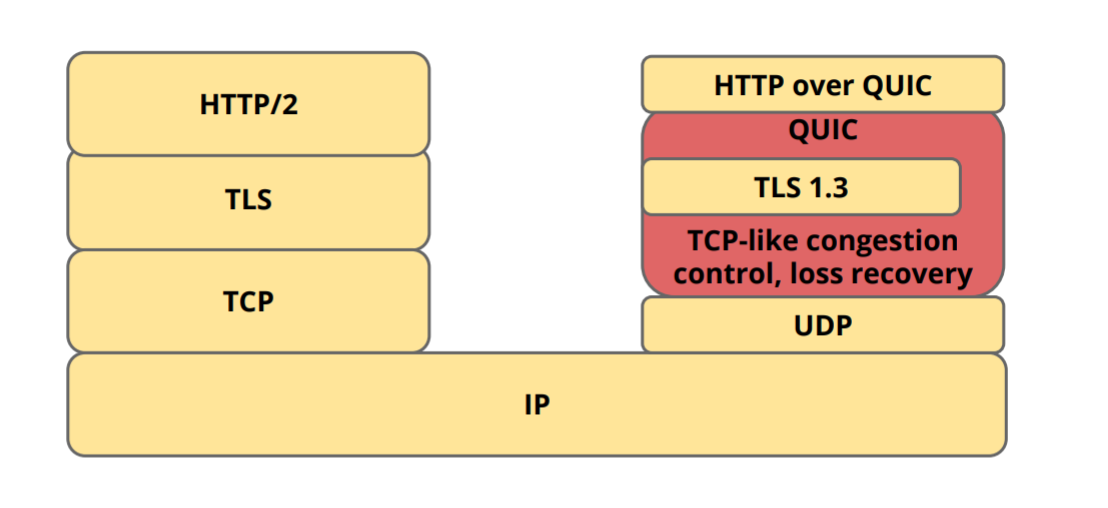
\includegraphics[width=0.9\textwidth]{figs/QUIC_network_stack.PNG}
    \caption{\texttt{QUIC/UDP/IP} network stack compared to \texttt{TCP/IP} network stack. This diagram is taken from \texttt{IETF} presentation about \texttt{QUIC} \cite{IETF_presentation_about_QUIC}.}
    \label{fig:QUIC_network_stack}
    \end{figure}

% [TODO: WHAT end-to-end LATENCY?]
One of the key ideas of QUIC is that it aims to reduce end-to-end latency by combining handshakes of both transport (\texttt{QUIC}) and security (\texttt{TLS1.3}) layers \cite{Google_QUIC_protocol_moving_the_web_from_TCP_to_UDP}, \cite{HTTP_3_the_past_the_present_and_the_future}. Hence, for this reason \texttt{TLS1.3} layer in Figure~\ref{fig:QUIC_network_stack} is shown as being part of the QUIC protocol. 
[TODO: fix this jump of ideas]
As Mattias Geniar said \cite{Google_QUIC_protocol_moving_the_web_from_TCP_to_UDP},
\texttt{HTTP over QUIC} layer (which is now called \texttt{HTTP/3} \cite{HTTP_3_the_past_the_present_and_the_future}) is smaller than analogous \texttt{HTTP/2} layer because stream multiplexing and connection management tasks are delegated to \texttt{QUIC} \cite{bib_grigorik2013}.
Similarly, the \texttt{UDP} layer is smaller than the \texttt{TCP} layer because \texttt{UDP} does not provide congestion control. 
In other words, \texttt{UDP} sends packets in \enquote{fire and forget} manner \cite{Google_QUIC_protocol_moving_the_web_from_TCP_to_UDP}.


\subsection{List of QUIC Features}
% https://archive.nanog.org/sites/default/files/meetings/NANOG64/1051/20150603_Rogan_Quic_Next_Generation_v1.pdf
% TODO: read https://tools.ietf.org/html/draft-ietf-quic-transport-32#section-1
% TODO: read https://arxiv.org/pdf/1801.05168.pdf
\begin{itemize}


 \item \textbf{Connection migration} 
 % (https://peering.google.com/\#/learn-more/quic, https://ma.ttias.be/googles-quic-protocol-moving-web-tcp-udp/)
 
    As I have already mentioned in the Introduction section, more than 90\% of all Internet users use mobile devices to connect to the Web \cite{bib_number_of_mobile_users}.
    An important aspect of portable devices is that their location, and thus Internet access point, can change relatively frequently \cite{PollardBarry2019HiAP}.
    This is particularly problematic for \texttt{TCP} because \texttt{TCP's} connection is tied to a particular \texttt{IP} address \cite{PollardBarry2019HiAP}.
    As a result, \texttt{TCP} needs to establish a new connection every time the network access point is changed \cite{PollardBarry2019HiAP}.
    This means that frequent access point changes would hurt \texttt{TCP's} performance because \texttt{TCP} would have to spend more time in the \enquote{slow-start} phase and perform additional handshakes.
    This example demonstrates that \texttt{TCP} protocol is old as it assumed that \texttt{IP} address would not frequently change \cite{PollardBarry2019HiAP}.
    In contrast, \texttt{QUIC} is more suitable to handle connections via mobile devices.
    In particular, \texttt{QUIC} has an explicit connection ID that does not depend on the IP address \cite{PollardBarry2019HiAP}.
    Hence, \texttt{QUIC} clients can migrate between multiple networks without having to re-establish a \texttt{QUIC} connection.
    
    
    





\item \textbf{Fast \texttt{TLS1.3} handshake}

As shown in Figure~\ref{fig:QUIC_handshake_vs_TCP-TLS_handshake}, one of the primary innovations of \texttt{QUIC} is that it combines transport and security layer handshakes.


     \begin{figure}[H]
    \centering
    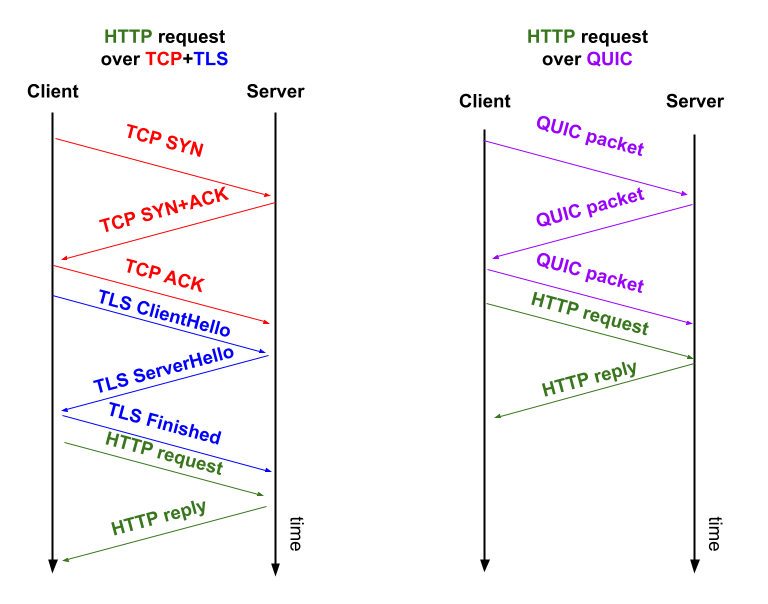
\includegraphics[width=0.9\textwidth]{figs/QUIC_handshake_vs_TCP-TLS_handshake.png}
    \caption{Comparison of handshakes required to issue an \texttt{HTTP} request. The left section demonstrates that traditionally multiple round trip times are required to establish a connection to issue an \texttt{HTTP} request. The right section of the diagram shows that \texttt{QUIC}, on the other hand, combines transport and security layer handshakes. This diagram is a reproduction of the similar diagram taken from \cite{the-road-to-quic}.}
    \label{fig:QUIC_handshake_vs_TCP-TLS_handshake}
    \end{figure}
 
 % TODO: Why do we need a TCP handshake?
 % TODO: why do we need a TLS handshake?
 % TODO: what info is sent in QUIC handshake?
 % MAYBE TODO: mention possible amplification attacks of QUIC (https://blog.cloudflare.com/the-road-to-quic/) 
 



  \item TODO zero RTT handshake
  
  
 
  \item \textbf{Reliability and  congestion control}
  
    \texttt{QUIC} also provides reliable data delivery because the main purpose of it is to replace \texttt{TCP} \cite{ietf-quic-transport-draft} by offering identical or better guarantees. 
    Similarly, \texttt{QUIC} implements congestion control because, as I have already mentioned in the previous sections, the underlying transport protocol layer \texttt{UDP} does not provide this mechanism. 
  
 

 
  \item Another feature of \texttt{QUIC} is that it uses \textbf{encryption by default} \cite{the-road-to-quic}.
  % TODO
  [TODO: add a source saying that now ISPs don't support QUIC without embeded security layer].
  However, there is some criticism that Internet Service Providers could be having problems in the future managing encrypted, and thus non-transparent, \texttt{QUIC} traffic inside their networks \cite{why-is-googles-quic-leaving-network-operators-in-the-dark}.
  
  \item TODO loss recovery
  
  \item TODO multiplexed streams
 
  \item TODO loss detection with signaling (using new seq number)
  
  
\end{itemize}


\subsection{Advantages of \texttt{QUIC}} \label{QUIC_advantages}

\begin{itemize}
  \item Reduced latency:
  According to [https://blog.chromium.org/2015/04/a-quic-update-on-googles-experimental.html]: "$<\ldots>$ QUIC outshines TCP under poor network conditions, shaving a full second off the Google Search page load time for the slowest 1\% of connections".
  \item TODO mention combined handshakes of transport and security layer protocols 
  % TODO: read https://blog.cloudflare.com/introducing-0-rtt/

  \item TODO solved \texttt{TCP} head-of-line blocking

  
  \item TODO mention how QUIC solves the problem of ossification
  
  \item TODO include https://blog.cloudflare.com/http-3-vs-http-2/
\end{itemize}




\subsection{\texttt{QUIC}'s Header Format} \label{subsection_QUIC_header_format}

\begin{itemize}
  \item TODO mention that the packet header encryption is separate from payload encryption
  \item TODO explain why do we need this separation
  \item TODO present long and short headers give a list of fields
  \item TODO mention that packet numbers are encrypted, but connection ID is not
\end{itemize}

\subsection{\texttt{QUIC}'s Adoption}

At the time of writing, $5.0\%$ of all the websites on the Internet used \texttt{QUIC} and $14.5\%$ used \texttt{HTTP/3} \cite{bib_Adoption_comparison_Between_http2_http3_quic}
(see Figure~\ref{fig:Adoption_comparison_Between_http2_http3_quic}).
However, as Matt Joras, Software Engineer from \texttt{Facebook}, said on the \texttt{Slack} chat of QUIC developers, the number of websites using \texttt{HTTP/3} does not correctly represent the protocol usage in terms of traffic. 
Hence, this diagram only demonstrates that \texttt{QUIC} is still in the relatively early deployment phase.

[TODO: add another analysis which calculates QUIC traffic]
[TODO: include https://radar.cloudflare.com/]


    \begin{figure}[ht]
    \centering
    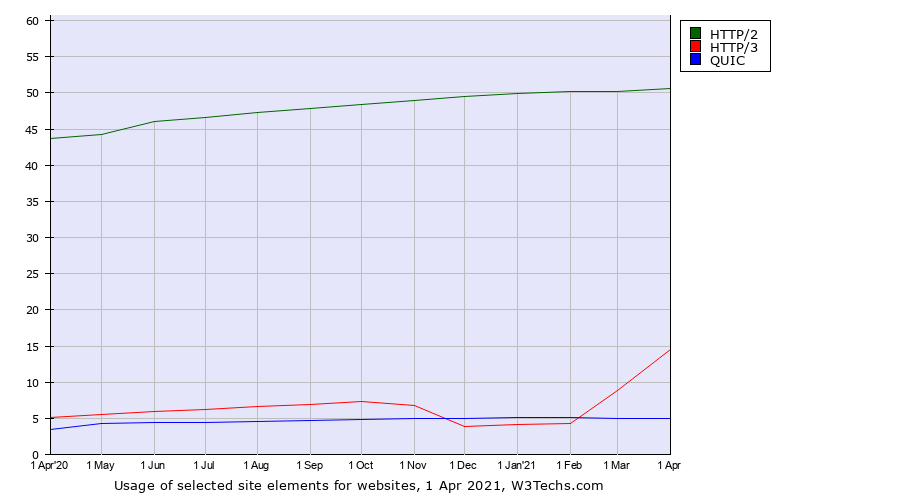
\includegraphics[width=0.9\textwidth]{figs/Adoption_comparison_Between_http2_http3_quic.png}
    \caption{Proportion of websites using \texttt{QUIC}, \texttt{HTTP/2} or \texttt{HTTP/3}. This diagram is taken from \cite{bib_Adoption_comparison_Between_http2_http3_quic}.}
    \label{fig:Adoption_comparison_Between_http2_http3_quic}
    \end{figure}









\section{Implementations of QUIC}

\subsection{List of QUIC's Implementations} \label{List_of_QUIC_implementations}
According to QUIC Working Group \cite{number_of_QUIC_implementations}, there is 31 different implementation of QUIC. Most of the implementations, 22 to be precise, are written using C/C++ language family (e.g. \texttt{Chromium}\footnote{https://chromium.googlesource.com/chromium/src/net/+/master/quic/}) while remaining implementations use Rust (e.g. \texttt{quiche}\footnote{https://github.com/cloudflare/quiche}), Python (e.g. \texttt{aioquic}\footnote{https://github.com/aiortc/aioquic}), Haskel (e.g. \texttt{Haskell quic}\footnote{https://github.com/kazu-yamamoto/quic}), Java (e.g. \texttt{kwik}\footnote{https://bitbucket.org/pjtr/kwik/src/master/}), Go (e.g. \texttt{quic-go}\footnote{https://github.com/lucas-clemente/quic-go}) or JavaScript (e.g. \texttt{Node.js QUIC}\footnote{https://github.com/nodejs/quic}).


\subsection{Why are there so many Implementations of QUIC?}

As I have already mentioned in the previous sections, \texttt{QUIC} is implemented in the user-space.
Hence, this flexibility simplifies the development and deployment of the new \texttt{QUIC} implementations.
However, there is an associated cost of using protocol written in user space - as Adam Langley and his colleagues noted \cite{QUIC_SERVER_REQUIRES_3-5_more_CPU_resources}, \texttt{QUIC} server required 3.5 more \texttt{CPU} resources.

\subsection{Why did I choose  \texttt{ngtcp2}?}
%TODO: fix style and grammar:
There are many implementations of QUIC (see subsection \ref{List_of_QUIC_implementations}) written in different languages.
I considered  \texttt{aioquic}\footnote{https://github.com/aiortc/aioquic},  \texttt{MsQuic}\footnote{https://github.com/microsoft/msquic},  \texttt{ngtcp2}\footnote{https://github.com/ngtcp2/ngtcp2},  \texttt{mvfst}\footnote{https://github.com/facebookincubator/mvfst} and \texttt{Quant}\footnote{https://github.com/NTAP/quant}.
Before changing the direction of the dissertation, one of the primary goals of the project was to turn off header encryption of QUIC packets so that I could inspect these packets in hardware.
Hence, I performed a survey to find \texttt{QUIC} implementation, which had an API to control encryption. 
\texttt{Aioquic}, \texttt{MsQuic} and \texttt{ngtcp2} seemed to be the most promising.
However, despite being a simple and well-documented implementation of \texttt{QUIC}, aioquic did not have an active development team that could answer technical questions.
Similarly, MsQuic seemed promising, but some of the performance measurement tools used by the \texttt{MsQuic} team were proprietary and not yet released to the public.
As this project is based on a paper written by Gianni Antichi and his colleagues \cite{Making_QUIC_Quicker}, I thought that it would be wise to use similar testing conditions in this dissertation too.
In particular, Gianni and his team evaluated several \texttt{QUIC} implementations, which were written in C or C++.
Hence, I decided to follow a similar approach, and I picked \texttt{ngtcp2}, which is also written in C.
Later on, I figured out that there is an experimental QUIC benchmarking tool called \texttt{h2load}\footnote{https://github.com/nghttp2/nghttp2/tree/quic}, which is compatible with \texttt{ngtcp2}.
Moreover, \texttt{h2load} is written by Mr Tatsuhiro  Tsujikawa (the co-author of \texttt{ngtcp2}).


\section{Requirements Analysis}
% TODO what is the purpose of this section?


\section{Starting Point}
As mentioned in the previous sections, this project builds on top of \texttt{ngtcp2} implementation of \texttt{QUIC}.
In other words, relevant networking stack tools such as cryptographic library (e.g. \texttt{OpenSSL}), benchmarking tool (e.g. \texttt{h2load}), custom \texttt{HTTP} layers (e.g. \texttt{nghttp2} and \texttt{ngtcp3}) have already been built and integrated. 
Similarly, the concept of QUIC was introduced in the Part IB \enquote{Computer Networking} course and fundamentals of C and C++ were covered in \enquote{Programming in C and C++} course. 
In addition, I used C++11 in my summer internship.

% TODO
[TODO: reference the starting point section from the initial project proposal]

\section{Software Engineering Techniques and Tools}
    To track the code changes, I used \texttt{Git} source control tool.
    In particular, I used \texttt{GitHub} to store forked repositories of \texttt{ngtcp2}, \texttt{openssl}, \texttt{nghttp2} and \texttt{nghttp3}.
    In addition, the dissertation document was written using online \LaTeX  editor called Overleaf\footnote{\url{https://www.overleaf.com/}} and changes were also committed to a separate repository on \texttt{GitHub}.
    Furthermore, I used different coding environments.
    At first, I worked with \texttt{NetBeans} IDE.
    But as I was extensively analysing existing code written by other programmers (i.e. \texttt{ngtcp2} and its related components), I needed an effective tool to search through the codebase.
    Hence, I opted for \texttt{Visual Studio Code} IDE which also had a convenient tool to compare \texttt{git} changes.
    
    
    Throughout the project, I tried to employ \texttt{Agile} software development practices.
    For instance, for performance evaluation, I had to configure testing machines using repetitive commands but typing these instructions by hand is a laborious and error-prone process.
    As a result, after detecting an error caused by an incorrect configuration, I usually augmented the \texttt{bash} setup script to set missing parameters automatically.
    Furthermore, I had Weekly progress updates with several other Part II students.
    During these virtual \enquote{stand-up meetings} I had an opportunity to reflect on project-related issues.
    To record my daily progress, I used a logbook, stored in the \texttt{Google Docs}.
    Besides that, I used an application called \texttt{Trello}\footnote{\url{https://trello.com/en-GB}} to group, track and re-order subtasks according to their importance (see Figure~\ref{fig:Trello_board}).

    \begin{figure}[ht]
    \centering
    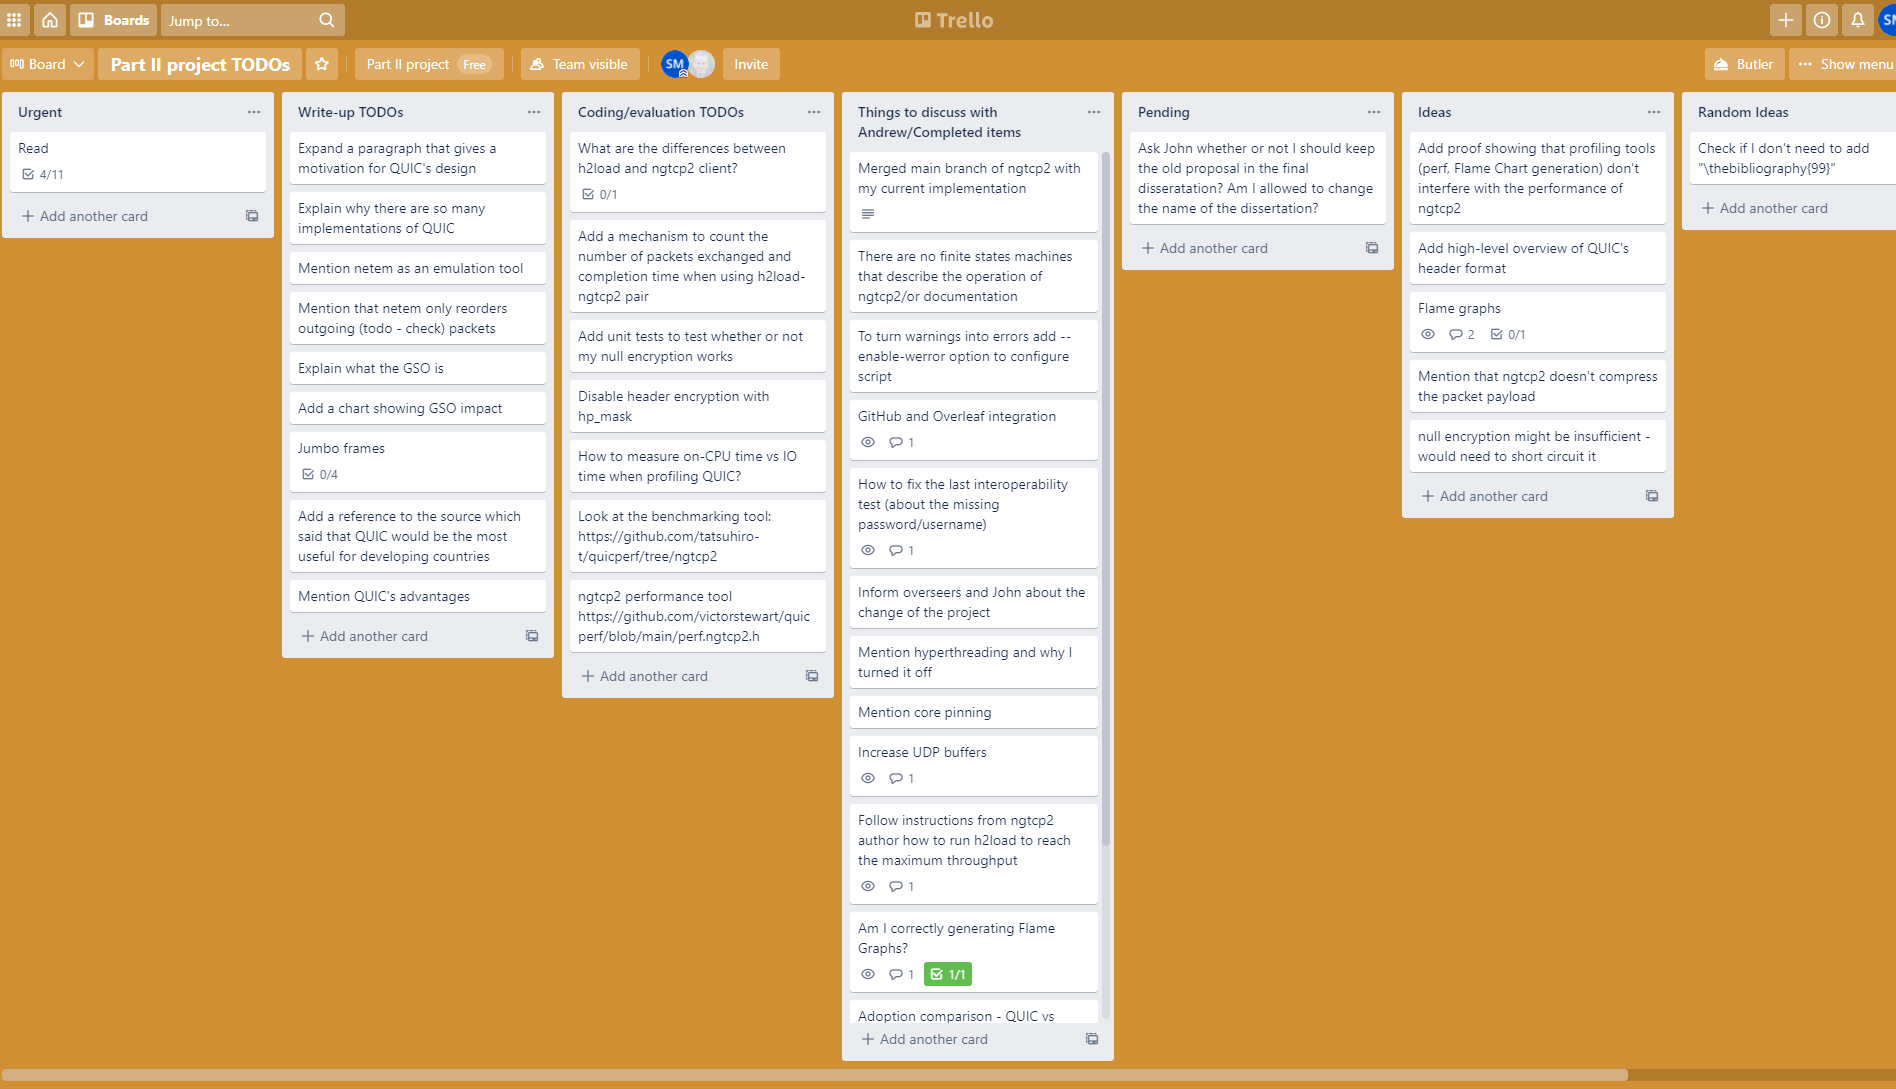
\includegraphics[width=0.9\textwidth]{figs/Trello_board.PNG}
    \caption{\texttt{Trello} board of important tasks}
    \label{fig:Trello_board}
    \end{figure}
    
    During the winter vacation I returned back home so I had made the necessary steps beforehand to be able to have remote access to the specialised hardware.
    In particular, I first enabled permanent remote access to the testing machines using remote desktop access software called \texttt{TeamViewer}\footnote{\url{https://www.teamviewer.com/en/}}.
    It allowed me to access the aforementioned machines outside the college network.
    Then, as shown in Figure~\ref{fig:setup_map}, I added additional redundant backup \texttt{ssh} connections between the testing computers to improve the resilience of the system in case one of the \texttt{TeamViewer} links failed.
    Finally, to further mitigate potential risks, I had two emergency contacts (two non-technical students from the same college) who were granted a permission to enter my room and access the machines inside it in case of an accident.
    This last step turned out to be useful because I was able to ask my fellow students to turn off the testing machines before the college network was shut down for maintenance operations.
    

    \begin{figure}[ht]
    \centering
    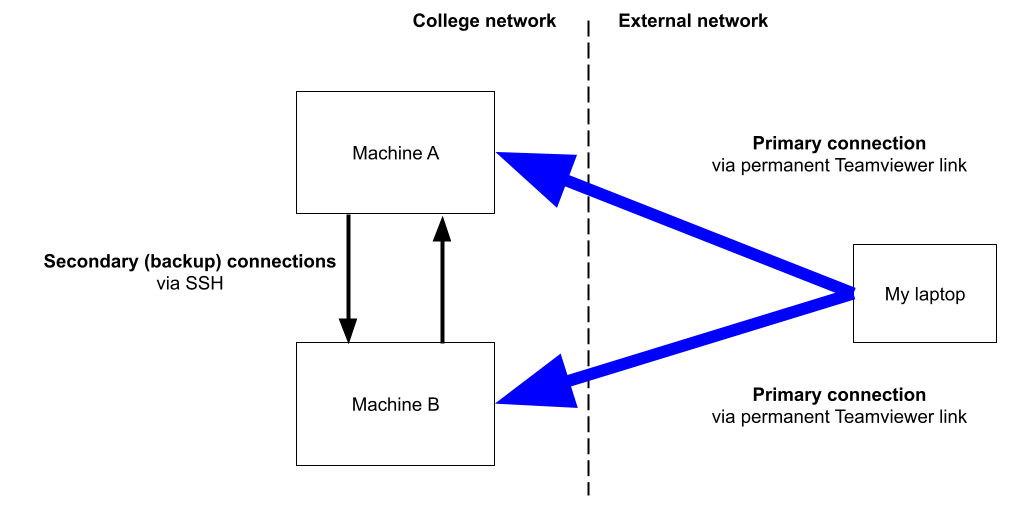
\includegraphics[width=0.9\textwidth]{figs/Setup map.png}
    \caption{Contingency plan to work remotely}
    \label{fig:setup_map}
    \end{figure}

    Besides that, I used different communication channels to discuss configuration and technical issues with other \texttt{QUIC} developers.
    At first, I used \texttt{GitHub} to raise issues.
    Then, I started using a direct messaging application called \texttt{Slack}\footnote{\url{https://slack.com/intl/en-gb/}} 
    and it improved the speed of communications substantially.

    Furthermore, after winter vacation, I brought an additional laptop from home to improve the development speed.
    This computer was used as a sandbox to test different implementations of \texttt{QUIC} before deploying them to the main machines.
    Before then, I had a problem that testing machines had pre-configured software which used incompatible settings with the configuration parameters required for \texttt{QUIC} implementations (e.g. existing software stack used older OS version).
    However, with the help of the additional laptop, I was able to verify the correctness of \texttt{ngtcp2}, a selected implementation of \texttt{QUIC}.
    Besides that, I ensured the correctness of the null encryption of \texttt{ngtcp2} by writing and running several integration tests.
    In particular, these tests check whether or not the received \texttt{HTML} file is identical to the transmitted \texttt{HTML} file.
    
    Finally, for some aspects of the project, I used non-standard or not recommended practices.
    For example, I ran testing machines with root privileges.
    On the one hand, such a configuration would be insecure for the general computer user. On the other hand, using root privileges by default allowed me to avoid frequent issues with insufficient permissions as I had to run configuration commands which required top-level permissions multiple times.
    
    

\chapter{Implementation}
% ------------------------------------------------
% TODO

%This chapter should describe what was actually produced: the programs which were written, the hardware which was built or the theory which was developed. Any design strategies that looked ahead to the testing stage should be described in order to demonstrate a professional approach was taken.

%Descriptions of programs may include fragments of high-level code but large chunks of code are usually best left to appendices or omitted altogether. Analogous advice applies to circuit diagrams or detailed steps in a machine-checked proof.

%The implementation chapter should include a section labelled "Repository Overview". The repository overview should be around one page in length and should describe the high-level structure of the source code found in your source code repository. It should describe whether the code was written from scratch or if it built on an existing project or tutorial. Making effective use of powerful tools and pre-existing code is often laudable, and will count to your credit if properly reported. Nevertheless, as in the rest of the dissertation, it is essential to draw attention to the parts of the work which are not your own. 

%It should not be necessary to give a day-by-day account of the progress of the work but major milestones may sometimes be highlighted with advantage.


% FROM: https://www.cst.cam.ac.uk/teaching/part-ii/projects/assessment
%Contribution to the field.
%Application of extra-curricular reading and original interpretation of previous work from academia or industry.
%Challenging goals and substantial deliverables with excellent selection and application of appropriate mathematical, scientific and/or engineering techniques.
%Clear and justified repository overview.
%At most minor faults in execution or understanding.
% ------------------------------------------------


In this chapter I first give an overview of the repository structure.


\section{Repository Overview} 
% TODO
[TODO add reference to the original page of ngtcp2]
First of all, I added support of null encryption in the cloned repository of \texttt{ngtcp2}.

In addition, I augmented \enquote{README} file of the primary repository with specific instructions on how to compile and run the software stack required for this project.

% TODO
[TODO: mention that I forked part of networking stack required to run ngtcp2. In particular, I worked on a separate openssl(embeded security layer), ngtcp2 (transport layer), nghttp2 and nghttp3 (application layers) ]

\section{Preparation scripts}
As I have already mentioned, I wrote several scripts to prepare testing machines for performance analysis.
These commands are stored in \texttt{\textasciitilde/.zshrc} and \texttt{\textasciitilde/.bashrc} files (see Appendix~\ref{preparation_script_from_zshrc}) meaning that preparation scripts are executed every time a new terminal is opened.


 % TODO mention ping test
 % TODO state that it configures virtual namespaces to separate server from client
 % TODO add scripts to appendix

The automatic preparation scripts improved development speed because certain repetitive tasks were automated.
Furthermore, the setup of the testing environment became more predictable, meaning that performance tests generated more reproducible results.



\section{Using Null Encryption}
% TODO
[TODO add reference saying that encryption of QUIC is turned on by default]

By design, QUIC uses encryption by default.
It encrypts both the payloads of the packets and some fields in the packet headers.


However, encryption and decryption operations were found to be computationally expensive.
% TODO
[TODO add a reference showing that QUIC crypto functions are expensive]

These intensive operations could have become a performance bottleneck of QUIC.
To validate this claim, I had to measure the impact of cryptographic operations on QUIC's performance by comparing the throughput between the two server-client pairs.
One pair had to use standard encryption and decryption procedures, while another had to exchange unencrypted packets.
I achieved this by implementing logic that can turn on null encryption on \texttt{ngtcp2}.
% TODO
[TODO add a link to null encryption]

In essence, null encryption is a technique that effectively turns off encryption by encrypting/decrypting the data by ``XOR"ing the data with a key made entirely of zeroes (which leaves the data unchanged). 

% TODO
[TODO - say which cryptographic operations are performed and which ones are omitted when using my implementation of null-crypto]


% TODO
[TODO: mention improved null encryption]

% TODO
[TODO: mention that I later on found existing null encryption and decryption mechanisms in the unit tests of \texttt{ngtcp2}. 
However, my implementation was developed independently and without knowledge about the existence of these functions.
This can be proven by my commit history and communication history on the \texttt{Slack} messaging platform.
Furthermore, the performance analysis I described before allowed me to identify potential bottlenecks of my implementation.
Hence, I was able to improve my null cryptographic operations in a systematic way.]





\section{Testing scripts}
% TODO
[TODO describe the structure and design of testing scripts (Python invokes bash scripts $>$ extracts data $>$ saves/aggregates data)]

% TODO
[TODO mention that machine A controls machine B via ssh]

\chapter{Evaluation}
% ------------------------------------------------
%This is where Assessors will be looking for signs of success and for evidence of thorough and systematic evaluation. Sample output, tables of timings and photographs of workstation screens, oscilloscope traces or circuit boards may be included. Care should be employed to take a professional approach throughout. For example, a graph that does not indicate confidence intervals will generally leave a professional scientist with a negative impression. As with code, voluminous examples of sample output are usually best left to appendices or omitted altogether.

%There are some obvious questions which this chapter will address. How many of the original goals were achieved? Were they proved to have been achieved? Did the program, hardware, or theory really work?

%Assessors are well aware that large programs will very likely include some residual bugs. It should always be possible to demonstrate that a program works in simple cases and it is instructive to demonstrate how close it is to working in a really ambitious case.
% ------------------------------------------------



\section{Setup}

As this project builds on the ideas presented in \cite{Making_QUIC_Quicker}, I thought that it would be reasonable to replicate a similar testing environment to obtain comparable results.

\subsection{Logical Setup}
To test a simple single flow performance, it is sufficient to have a single \texttt{QUIC} server-client pair, as depicted in Figure~\ref{fig:Logical_testing_environment}.
To measure \texttt{QUIC} performance under different conditions, we need to add a network emulator between the \texttt{QUIC} client and the \texttt{QUIC} server.

    \begin{figure}[ht]
    \centering
    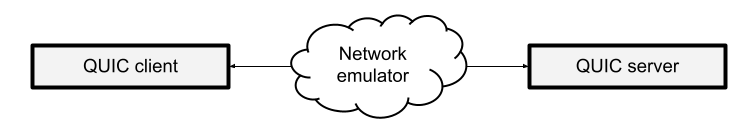
\includegraphics[width=0.9\textwidth]{figs/Logical_testing_environment.png}
    \caption{Logical configuration of testing environment}
    \label{fig:Logical_testing_environment}
    \end{figure}

\subsection{Physical Setup}
    In the ideal scenario, we might want to use three dedicated machines for performance measurements, as shown in the previous section.
    However, I decided to use a slightly different physical layout (see Figure~\ref{fig:Physical_testing_environment}).
    In this environment, one machine (A) hosts client-server pair, while another computer (B) acts as a network emulator.
    The physical configuration differs from the logical configuration because I wanted to replicate testing conditions under which Gianni Antichi and his colleagues performed throughput measurements of QUIC \cite{Making_QUIC_Quicker}.
    One advantage of having both server and client running on the same machine is that the shared system clock can perform measurements more accurately. 
    

    \begin{figure}[ht]
    \centering
    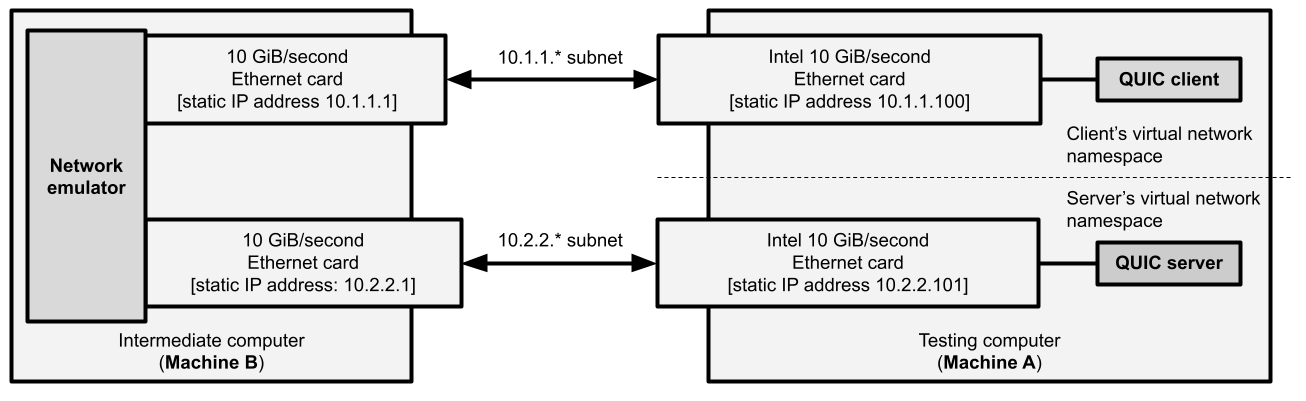
\includegraphics[width=0.9\textwidth]{figs/Physical_testing_environment.png}
    \caption{Physical configuration of testing environment. This scheme is an adaptation of the configuration environment used in  \cite{Making_QUIC_Quicker}}
    \label{fig:Physical_testing_environment}
    \end{figure}
    
    As we can see from Figure~\ref{fig:Physical_testing_environment}, both \texttt{QUIC} client and server operate on different virtual network namespaces which do not have shared point-to-point links.
    Client and server are assigned different network subnets.
    An intermediate machine (B) is configured as the default gateway for both virtual network namespaces.
    As a result, all the packets between the \texttt{QUIC} server and client have to travel via an intermediate machine (B).
    Here, depending on the experiment, network perturbations (e.g. packet loss, delay, reordering) may be introduced.
    In particular, to simulate different networking conditions I used \texttt{NetEm} tool (abbreviation of \enquote{Network Emulator})\footnote{http://manpages.ubuntu.com/manpages/trusty/man8/tc-netem.8.html}.
    The small implementation detail of \texttt{NetEm} is that by default it introduces traffic perturbations for the packets leaving the network interface but not the incoming packets \cite{Ubuntu_Manpage_NetEm}.
    Hence, to simulate symmetrical network conditions I had to specify \texttt{NetEm} rules for both interfaces of the intermediate machine.
    For this reason, in other diagrams, I represent Network Emulator as separated into two sections (see Figure~\ref{fig:Wireshark_separation}).
    
    
    IP forwarding is enabled on the intermediate machine (B), redirecting \texttt{QUIC} packets from one subnet to another.
    Correctness of the experimental environment was tested by inspecting transit packets on the machine B.

    The intermediate machine adds only limited overhead.
    I derived these conclusions by comparing round-trip-times (using \texttt{ping} tool) and the maximum available \texttt{UDP} throughput (using \texttt{iperf3} tool) under two different conditions.
    At first, I measured performance when packets travel from one physical interface of machine A to its another physical interface via machine B.
    Then, I performed identical tests but without the intermediate machine meaning that packets were still forced to go from one physical interface to another via a loopback cable.
    Results were as follows: the maximum \texttt{UDP} throughput via machine B was 4.11 Gbits/sec [TODO: redo experiment] and via loopback cables this number was 9.91 Gbits/sec.
    In both case, throughput was measured on the receiver side.
    Similarly, after introducing the intermediate machine, the \texttt{RTT} increased from:
    
    \textbf{"RTT min/avg/max/mdev = 0.077/0.118/0.156/0.026 ms"}\\
    (\url{https://github.com/simonasmulevicius/Part-II-dissertation/blob/main/testing-scripts/test_overhead-of-intermediate-machine/test_maximum-iperf-troughput_via-loopback-cables/ping_result.txt})
    %[TODO: update these numbers with the new values from "test_ping-via-loopback-cables]
    
    to
    
    \textbf{"RTT min/avg/max/mdev = 0.188/0.262/0.353/0.065 ms"}\\
    (\url{https://github.com/simonasmulevicius/Part-II-dissertation/blob/main/testing-scripts/test_overhead-of-intermediate-machine/test_maximum-iperf-troughput_via-B/ping_result.txt})
    
    (Here each result was obtained after running ten \texttt{ping} experiments).
    
    % TODO
    [TODO: add a table of results showing that lower RTT of looback cables increased throughput of ngtcp-h2load by about 10\%]
    % https://github.com/simonasmulevicius/Part-II-dissertation/blob/main/testing-scripts/test_overhead-of-intermediate-machine/test_unencrypted-ngtcp2-throughput_via-loopback_delay-0ms_uncorrelated-loss-0_0_percent_improved-null-encryption_with-command-line-option/result.ods
    

    Similarly, \texttt{TCP} throughput via loopback cable was 9.89 Gbis/sec.
    [TODO: what was TCP throughput via machine B?]


    Large segmentation offload and \texttt{TCP} segmentation offload mechanisms were in place on the machine A. 


\section{Benchmarking tools}
% Frame pointer points to the top/bottom of the stack (from https://www.youtube.com/watch?v=nXaxk27zwlk&ab_channel=CppCon)
\subsection{iperf3}
\texttt{Iperf3} is a tool that generates artificial \texttt{TCP} or \texttt{UDP} traffic and thus measures throughput of these protocols.
\texttt{Iperf3} performs throughput measurements between \texttt{iperf3} server and client.
We can assume that \texttt{UDP}'s throughput is a theoretical maximum of \texttt{QUIC} throughput as \texttt{QUIC} builds on top of \texttt{UDP}.
However, \texttt{UDP} does not provide a similar set of guarantees as \texttt{QUIC} does.
For example, \texttt{UDP} does not guarantee reliable packet delivery so the sender and receiver could see different throughput values.
Hence, to put \texttt{QUIC} into the perspective, it is worth comparing its throughput against the throughput of the similar \texttt{TCP} protocol.
An important aspect of \texttt{TCP} is that its congestion control mechanism allows sender to discover an appropriate sending bitrate.
In contrast, \texttt{UDP} does not take into account the state of the network.
Consequently, if unlimited \texttt{UDP} throughput is allowed, then one could flood the network by running \texttt{iperf3} to measure \texttt{UDP} throughput.
However, as shown in Figure~\ref{fig:Wireshark_separation}, performance analysis tests were executed on the separate testing network so no damage was done to the public network.


% TODO
[TODO: mention that one can adjust UDP send or receive (TODO check which one) buffer size]



\subsection{ping}
\texttt{Ping} is a network analysis tool used to measure the round trip time between the two communicating parties.
As mentioned in \cite{internet-control-message-protocol-icmp}, \texttt{ping} uses Internet Control Message Protocol (or \texttt{ICMP} for short) to issue a request-reply pair.
Round trip time measurements were used to test the correctness of the testing environment (e.g. to measure additional network delay induced by the intermediate machine).
However, on \texttt{ping} could not be used to measure one-way delay because network delays can be asymmetric.


\subsection{Wireshark}

\texttt{Wireshark}\footnote{https://www.wireshark.org/} is a conventional tool used to inspect captured network packets (see Figure~\ref{fig:Wireshark_screenshot}).
\texttt{Wireshark} visualises key information about the packets - source and destination \texttt{IP} addresses, type of protocol and time when the packet was received on the specified network interface.

    \begin{figure}[H]
    \centering
    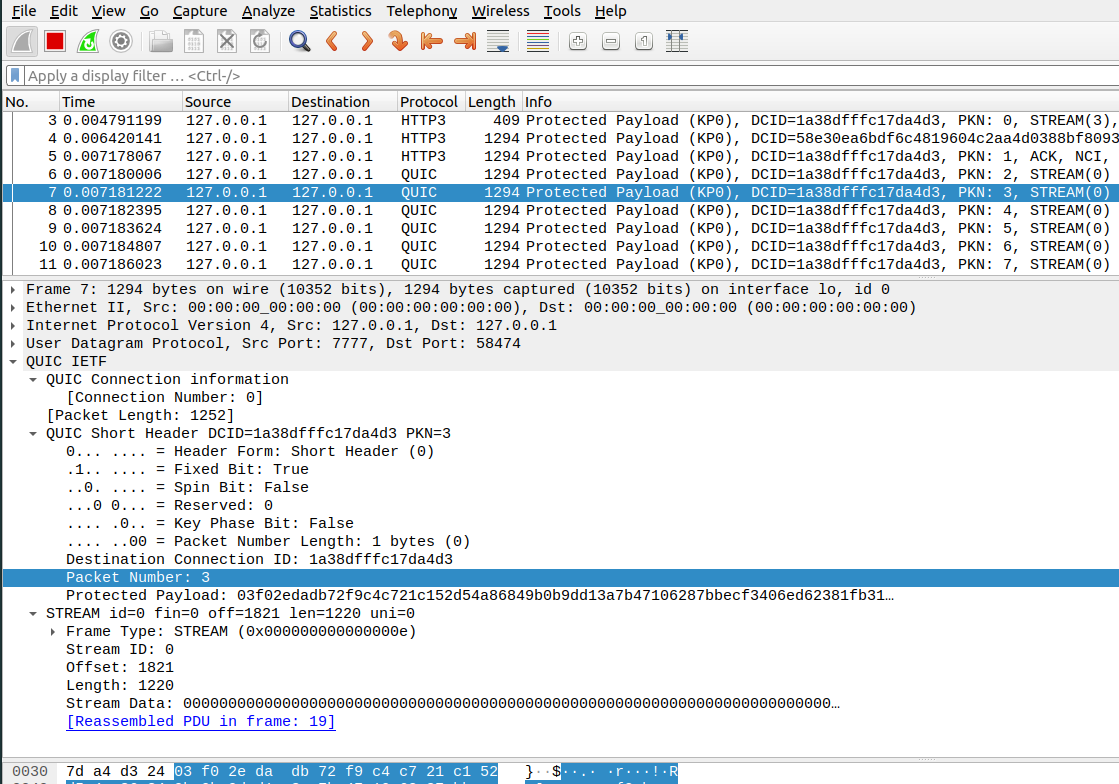
\includegraphics[width=0.95\textwidth]{figs/Wireshark_screenshot.png}
    \caption{\texttt{Wireshark} captured several \texttt{QUIC} packets whose numbers (abbreviated PKN) are decrypted and displayed on the right hand side.}
    \label{fig:Wireshark_screenshot}
    \end{figure}
    
When required, I ran \texttt{Wireshark} on the intermediate machine to inspect size of the packets transferred between the \texttt{QUIC} client and server.
It is worth mentioning that \texttt{QUIC} packets are encrypted.
Hence, I had to share server's cryptographic certificate with \texttt{Wireshark} so that it could decrypt and extract relevant fields (e.g. packet number) of observed \texttt{QUIC} packets.

I used \texttt{Wireshark} in an ethical manner meaning that I only used it to analyse traffic between the dedicated network interfaces.
In other words, as demonstrated in Figure~\ref{fig:Wireshark_separation}, I did not capture packets from the college network because testing environment used separate network interfaces. 

    \begin{figure}[H]
    \centering
    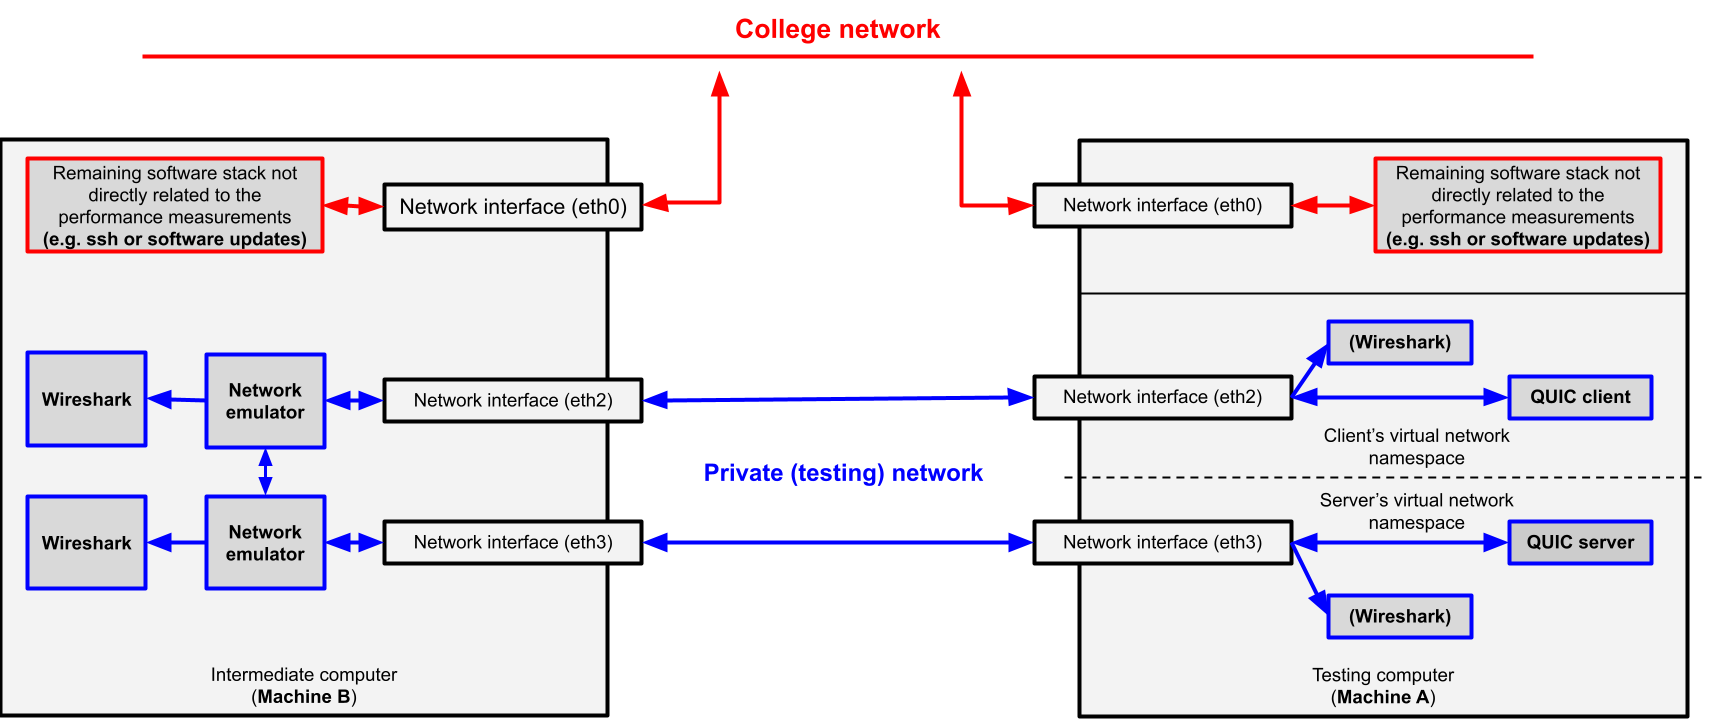
\includegraphics[width=0.95\textwidth]{figs/Wireshark_separation.png}
    \caption{Testing was performed on a private network. Hence, \texttt{Wireshark} was not used to capture packets from the college network}
    \label{fig:Wireshark_separation}
    \end{figure}



\subsection{perf}
\texttt{Perf}\footnote{https://perf.wiki.kernel.org/index.php/Main\_Page} is a performance analysis tool that measures CPU performance by sampling the call stack.

% TODO
[TODO: differentiate between sampling based mechanisms and another family of perf analysis tools[TODO what is the name of that group?]]

[TODO: limitations and overheads of sampling]

[TODO: describe the selection process of frequencies (why 997 and not 1000)]



\subsection{Flame Graphs}
\texttt{Flame Graphs} \footnote{\url{http://www.brendangregg.com/flamegraphs.html}} is a performance analysis tool which is used to visualise the performance of the program.
In this project I used CPU \texttt{Flame Graphs} that show the aggregated call stacks of numerous samples (see Figure~\ref{fig:perf_results_of_h2load}).
To understand the \texttt{Flame Graphs} we should first look at the simple example diagram (see Figure~\ref{fig:Flame_Graphs_explanation}).

    \begin{figure}[H]
    \centering
    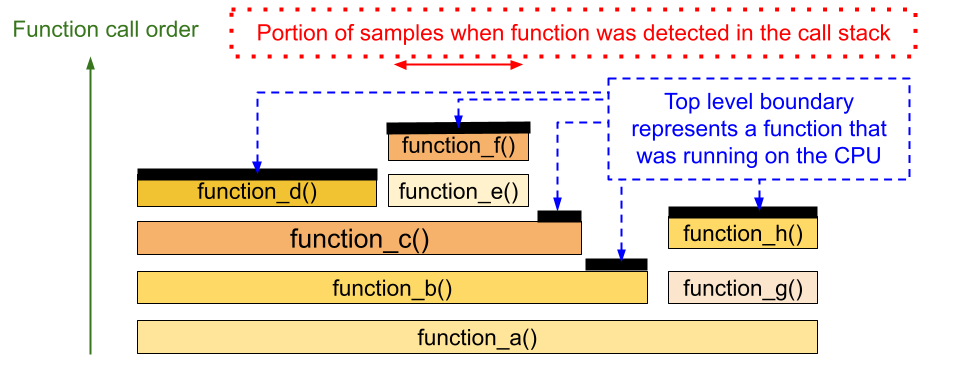
\includegraphics[width=0.9\textwidth]{figs/Flame_Graphs_explanation.png}
    \caption{Schematic diagram of \texttt{Flame Graphs} adopted from Brendan Gregg's presentation \cite{USENIX_ATC2017_flamegraphs}}
    \label{fig:Flame_Graphs_explanation}
    \end{figure}

Here y-axis of \texttt{Flame Graphs} represents the depth and frames of the call stack \cite{CPU_Flame_graphs}.
For instance, we can see in Figure~\ref{fig:Flame_Graphs_explanation} that \textbf{function\_a()} invoked function calls \textbf{function\_b()} and \textbf{function\_g()}. 
However, an important point to mention is that x-axis of \texttt{Flame Graphs} does not represent time \cite{CPU_Flame_graphs}.
Instead, function names are sorted alphabetically along the x-axis and it represents the approximate percentage of stack frames which were in the call stack \cite{CPU_Flame_graphs}.
Hence, by looking at Figure~\ref{fig:Flame_Graphs_explanation} we can tell that \textbf{function\_b()} and its \enquote{children} functions spent more time on CPU than \textbf{function\_g()} and its corresponding functions but we can not tell the relative order in which these functions were called.
Furthermore, in order to better identify the most frequent function calls, stack frames sampled at different times can be merged if they have a shared ancestor \cite{CPU_Flame_graphs}.
As a result, by looking at Figure~\ref{fig:Flame_Graphs_explanation} we can not differentiate whether or not function calls \textbf{function\_b()} and \textbf{function\_g()} did not interleave.

In the standard \texttt{Flame Graph}, different frames are coloured differently in order to increase visual contrast between the neighbouring cells in the diagram \cite{CPU_Flame_graphs} (see yellow, orange and red rows in Figure~\ref{fig:perf_results_of_h2load}).
However, in this project, I am also using \texttt{Differential Flame Graphs} that depict the difference between the two \texttt{Flame Graphs} \cite{Differential_Flame_Graphs}.
The structure of \texttt{Differential Flame Graph} is identical to the standard \texttt{Flame Graph} but the colouring information identifies which functions were more or less common in the second \texttt{Flame Graph} when compared with the reference \texttt{Flame Graph} \cite{Differential_Flame_Graphs}.

% TODO
[TODO: add an example of \texttt{Differential Flame Graph}]


% sampling based method



[MAYBE TODO: mention that I had to enable additional compiler flags to be able to see deeper call frames - before that they were optimised by compiler and some stacks were partially anonymous  -- add a reason why this problem occurred - compiler optimised one register?]

    \begin{figure}[ht]
    \centering
    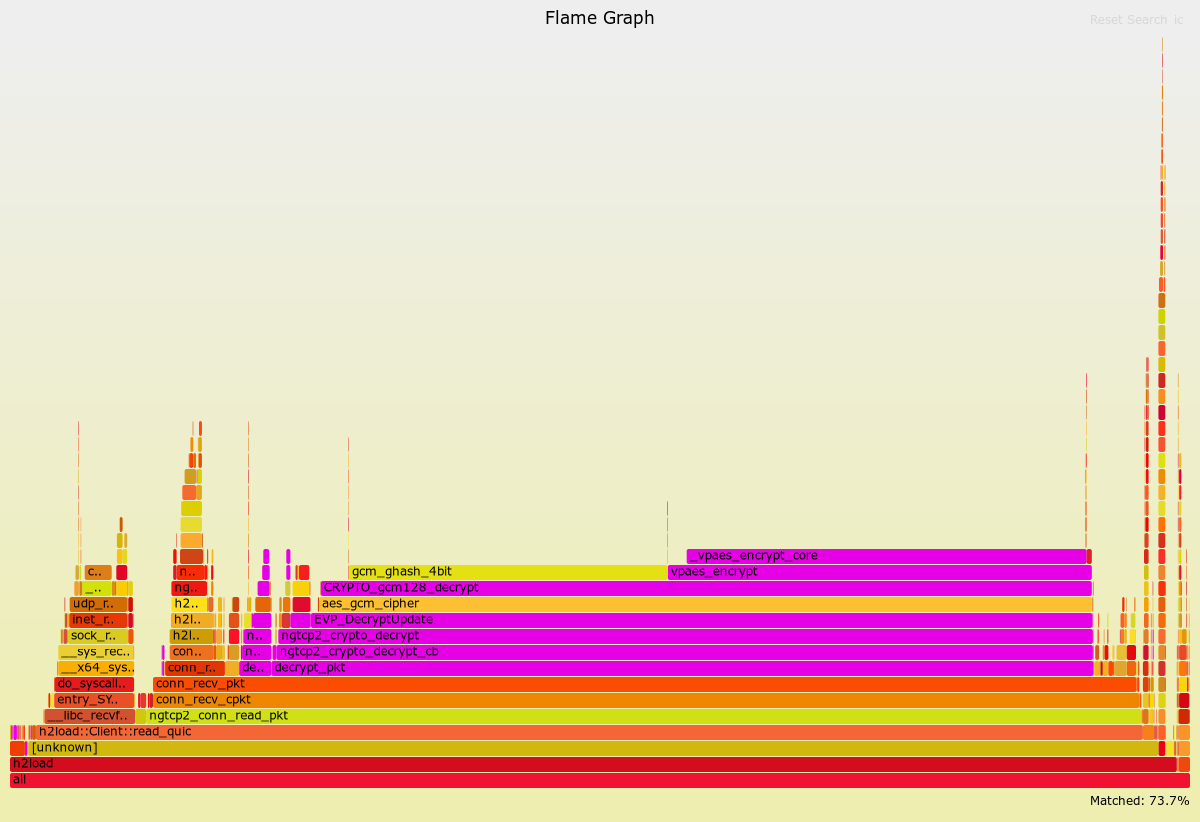
\includegraphics[width=0.9\textwidth]{figs/perf_results_of_h2load.png}
    \caption{Typical \texttt{perf} results of running \texttt{h2load} client against \texttt{ngtcp2} server on the same machine (A), when packets are transferred via an intermediate machine (B). This graph shows that about 70\% of the time, default \texttt{ngtcp2} version spends doing cryptographic operations} 
    \label{fig:perf_results_of_h2load}
    \end{figure}
    
\subsection{qlog and qvis}
% TODO
[TODO give a high-level overview of qlog format]

[TODO: why is it hard to visualise QUIC's behaviour?]



\section{Parameter Tuning}

\subsection{IP Version}

To make results comparable with older studies, I decided to disable IPv6 in the testing environment.
By specifying a particular IP version, we reduce the number of variable parameters.
Fortunately, at the time of writing, according to Google's IPv6 adoption tracker \cite{IPv6_Adoption_Statistics}, only a third of all Internet users (30-35 \% to be precise) use IPv6 to connect to Google's services.
Hence, analysis involving IPv4 is still relevant today.

%TODO
[TODO: Ubuntu 20.04 has different mechanism  to disable IPv6 - check that it is still working ]

\subsection{Hyper-threading}\label{Hyperthreading_Subsection_Tag}

As Michael E. Thomadakis states on the 23rd page of \cite{hyperthreading_book}, \texttt{hyper-threading} (more generally known as \texttt{simultaneous multi-threading}) is a thread allocation technique that allows two threads to run on the same physical core at the same time.
On the testing machines \texttt{hyper-threading} at first was implemented by assigning two virtual cores for every physical core (see Figure~\ref{fig:topology_with_hyperthreading}).
For instance, in this diagram core \enquote{L \#0} has two \enquote{processing units} marked as \enquote{PU L\#0} and \enquote{PU L\#1}.

    \begin{figure}[H]
    \centering
    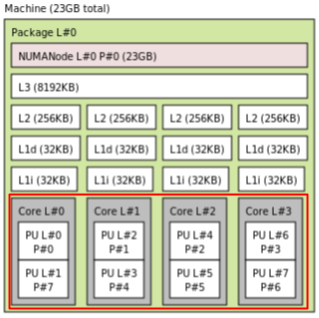
\includegraphics[width=0.8\textwidth]{figs/topology_with_hyperthreading.png}
    \caption{Memory topology of machine A when \texttt{hyper-threading} is turned on (Figure generated by \texttt{lstopo} command)}
    \label{fig:topology_with_hyperthreading}
    \end{figure}

As stated in \cite{hyperthreading_book}, this means that threads allocated to such virtual cores (also marked as \enquote{processing units} in the diagram above) would share the same physical resources (e.g. private L1 cache entries).
This is problematic for precise experiments.
On the one hand, a neighbouring thread might pre-fetch required data to the cache, but on the other hand, this thread might pollute the cache, thus hurting the performance of the thread which is being measured.
Hence, to reduce the potential performance variability, I had to disable \texttt{hyper-threading} on the testing machines.
The final version of architectural topology is shown in Figure~\ref{fig:memory_topology}. 
Correct configuration of \texttt{hyper-threading} was tested using different commands, such as \texttt{lscpu} and the aforementioned \texttt{lstopo}. 

    
    
\subsection{Separated Cores} \label{SeparatedCores_Subsection_Tag}
Machine A from Figure~\ref{fig:Physical_testing_environment} has four physical cores (see Figure~\ref{fig:memory_topology}).
To make performance tests even more predictable, I had to assign exclusive physical cores to the QUIC client and server using \texttt{taskset}\footnote{https://man7.org/linux/man-pages/man1/taskset.1.html} tool.
In particular, \texttt{ngtcp2} server was assigned the first core (marked as \enquote{P\#0} in Figure~\ref{fig:memory_topology}).
QUIC client (i.e. \texttt{ngtcp2} or \texttt{h2load} client) was assigned the second core (marked as \enquote{P\#1}).
Finally, remaining two cores (marked as \enquote{P\#2} and \enquote{P\#3}) were assigned to all the remaining system processes.
Robert Love refers to this technique of assigning particular processes to particular cores as \texttt{hard CPU affinity} \cite{CPU_Affinity}.

    \begin{figure}[H]
    \centering
    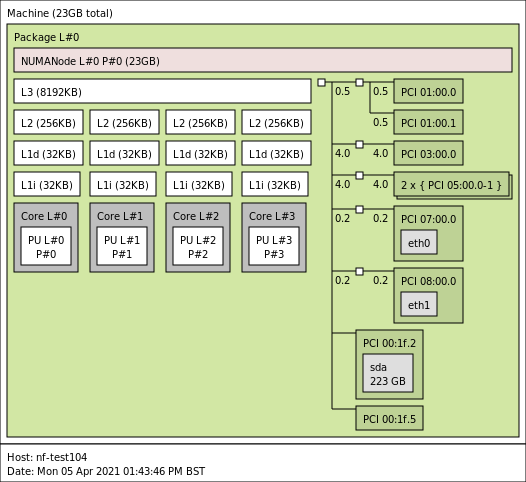
\includegraphics[width=0.8\textwidth]{figs/memory_topology.png}
    \caption{Memory topology of machine A  when \texttt{hyper-threading} is turned off (Figure generated by \texttt{lstopo} command)}
    \label{fig:memory_topology}
    \end{figure}

In addition, to evaluate the impact of core pinning, I measured throughput of \texttt{QUIC} under two different conditions by sending a file of the specified size over the intermediate machine.
At first, I allocated both \texttt{QUIC} server and client to the same core (see the red dashes in Figure~\ref{fig:Throughput_via_A-to-B-to-A_MTU=1500}).
Then, I performed identical throughput analysis tests with separated cores meaning that \texttt{QUIC} server and client resided on the two different cores.
Blue dashes in Figure~\ref{fig:Throughput_via_A-to-B-to-A_MTU=1500} demonstrate that core pinning almost doubled the maximum \texttt{QUIC} throughput for the transfer of large files (above 100MB).
However, impact of core pinning is not substantial when transferring small files.
One explanation of this could be that transmission time of small files is dominated by the overhead of networking stack and transmission time of a single packet.
As far as testing conditions are concerned, the intermediate machine was not configured to introduce additional explicit traffic perturbations.
    \begin{figure}[H]
    \centering
    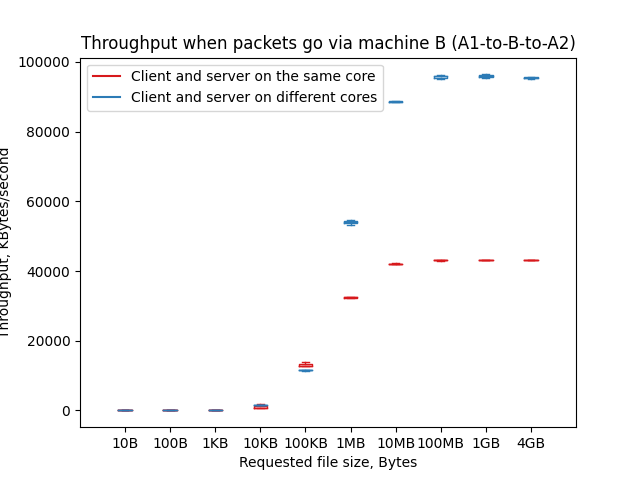
\includegraphics[width=0.8\textwidth]{figs/Throughput via node B (A-to-B-to-A)_MTU=1500.png}
    \caption{Impact of core pinning for \texttt{QUIC} throughput}
    \label{fig:Throughput_via_A-to-B-to-A_MTU=1500}
    \end{figure}

% TODO
[TODO add a chart showing lower performance variability when using different cores for testing ]

% TODO
[TODO according to https://www.kernel.org/doc/ols/2009/ols2009-pages-169-184.pdf, "CPU affinity" reduces cache misses]

\subsection{GSO}
\begin{itemize}
  \item TODO introduce GSO (General Segmentation Offload)
  
  
  \item TODO add a chart showing GSO's impact on throughput
  
  
  \item TODO mention when GSO is relevant
  
  \item TODO state that from now on, GSO is used in all the remaining tests by default because GSO provided great performance improvements
\end{itemize}

\subsection{MTUs}
\begin{itemize}
  \item TODO introduce/refresh MTUs
  \item TODO demonstrate the Jumbo frames impact for iperf/QUIC throughput
  
  
  
    \begin{figure}[H]
    \centering
    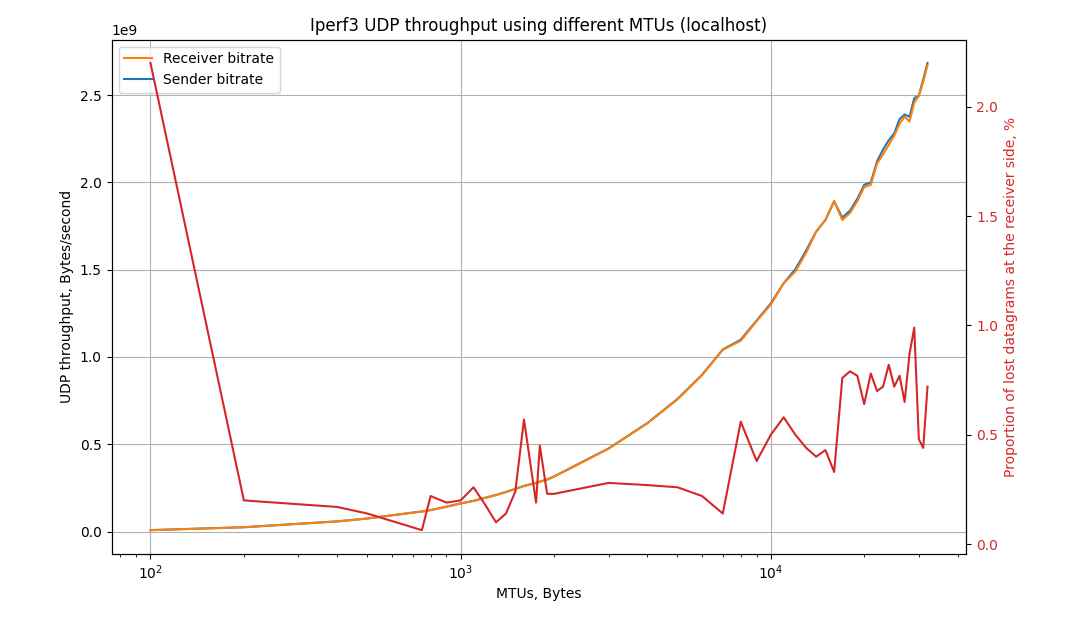
\includegraphics[width=0.9\textwidth]{figs/Iperf3 UDP throughput using different MTUs (localhost).png}
    \caption{Impact of MTU size for iperf throughput (when packets travel via localhost)}
    \label{fig:MTU_impact_for_localhost_iperf_throughput}
    \end{figure}
    
    \begin{figure}[H]
    \centering
    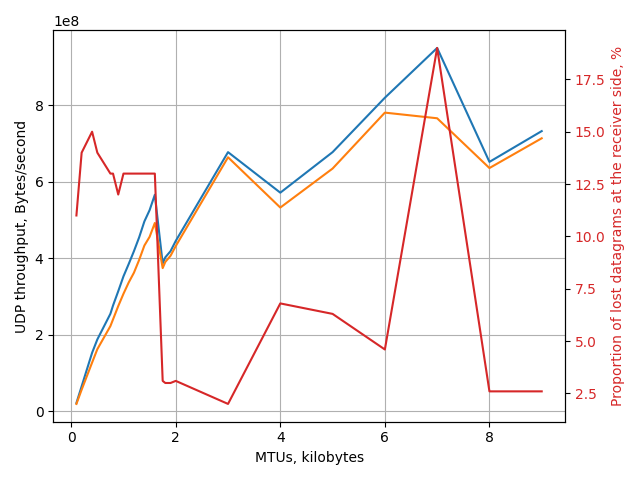
\includegraphics[width=0.9\textwidth]{figs/Iperf3 UDP throughput using different MTUs (A1-to-B-to-A2).png}
    \caption{Impact of MTU size for iperf throughput (when packets travel via the intermediate machine)}
    \label{fig:}
    \end{figure}
  
  
  
% Please add the following required packages to your document preamble:
% \usepackage{multirow}
\begin{table}[H]

    \begin{tabular}{|c|c|c|c|c|c|}
    \hline
    \multirow{2}{*}{MTU (B)} & \multirow{2}{*}{\begin{tabular}[c]{@{}c@{}}Requested\\ file size\end{tabular}} & \multicolumn{4}{c|}{Throughput (MiB/s)}                                                     \\ \cline{3-6} 
                             &                                                                                & minimum & maximum & mean    & \begin{tabular}[c]{@{}c@{}}standard \\ deviation\end{tabular} \\ \hline
    \multirow{2}{*}{1280}    & 1MB                                                                            & 40.610  & 47.870  & 44.125  & 2.487                                                         \\ \cline{2-6} 
                             & 1GB                                                                            & 98.990  & 105.200 & 103.950 & 1.794                                                         \\ \hline
    \multirow{2}{*}{1500}    & 1MB                                                                            & 42.060  & 50.220  & 45.382  & 2.547                                                         \\ \cline{2-6} 
                             & 1GB                                                                            & 107.920 & 110.820 & 110.001 & 0.942                                                         \\ \hline
    \multirow{2}{*}{9000}    & 1MB                                                                            & 37.300  & 46.950  & 39.750  & 2.727                                                         \\ \cline{2-6} 
                             & 1GB                                                                            & 135.940 & 141.500 & 139.616 & 1.852                                                         \\ \hline
    \end{tabular}


    \begin{tabular}{|c|c|c|c|c|c|}
    \hline
    \multirow{2}{*}{MTU (B)} & \multirow{2}{*}{\begin{tabular}[c]{@{}c@{}}Requested\\ file size\end{tabular}} & \multicolumn{4}{c|}{Completion time (s)}                                                 \\ \cline{3-6} 
                             &                                                                                & minimum & maximum & mean  & \begin{tabular}[c]{@{}c@{}}standard\\ deviation\end{tabular} \\ \hline
    \multirow{2}{*}{1280}    & 1MB                                                                            & 0.020   & 0.023   & 0.022 & 0.001                                                        \\ \cline{2-6} 
                             & 1GB                                                                            & 9.070   & 9.640   & 9.180 & 0.166                                                        \\ \hline
    \multirow{2}{*}{1500}    & 1MB                                                                            & 0.019   & 0.023   & 0.021 & 0.001                                                        \\ \cline{2-6} 
                             & 1GB                                                                            & 8.610   & 8.840   & 8.674 & 0.075                                                        \\ \hline
    \multirow{2}{*}{9000}    & 1MB                                                                            & 0.020   & 0.026   & 0.024 & 0.001                                                        \\ \cline{2-6} 
                             & 1GB                                                                            & 6.740   & 7.020   & 6.834 & 0.092                                                        \\ \hline
    \end{tabular}




    \centering
    \caption{Impact of Jumbo frames on the throughput of \texttt{ngtcp2} Completion time required to transfer specified files. In particular, this experiment measures QUIC throughput between the server and the client when they are pinned to two different cores on the same machine, and their packets travel via an intermediate machine (as demonstrated in Figure~\ref{fig:Physical_testing_environment}).
    Furthermore, a server uses a single thread, only a single stream is used, and a single file transfer is performed for each experiment.
    }
    \label{fig:Impact_of_Jumbo_frames_for_ngtcp2_throughput}
\end{table}

  
  \item TODO show that Jumbo frames are not accepted in the wild Internet / TODO state that MTUs above 1500 bytes are not prevalent in the Internet
  
  
  See Table~\ref{fig:Impact_of_Jumbo_frames_for_ngtcp2_throughput}.
  
  
\subsection{Interrupt Request Queue (IRQ) Balancing} 
Breno Henrique Leitao in his work suggested using \cite{Tuning_10Gb_network_cards_on_Linux} Interrupt Request Queue (IRQ) Balancing to improve general throughput of the testing system.
By default, \texttt{IRQ} is enabled meaning that operating system aims to distribute the burden of handling interrupts evenly over all the processors \cite{Tuning_10Gb_network_cards_on_Linux}.
The suggestion was to delegate processing of certain interrupts to specified processors hoping that this would improve performance of cores that were designated for the \texttt{QUIC} tests.
However, \texttt{IRQ} did not yield any noticeable effects for the \texttt{UDP} throughput measured by \texttt{iperf3} so I decided to leave the default \texttt{IRQ} settings on.
One plausible explanation for this insignificant improvement could be that the testing environment used already saturated network link.
In other words, measured maximum available throughput before and after experiment was around 9.8Gbits/second while the maximum theoretical limit of the link was 10Gbits/second. 


\subsection{Size of the buffers} 

% TODO
[TODO: 1. Update send and receive buffers according to: https://www.kernel.org/doc/ols/2009/ols2009-pages-169-184.pdf]  

[TODO: 2. State that adjusted buffers reduce UDP packet loss rate] 
 
 
  
\end{itemize}






\section{Impact of Cryptographic Operations}
% TODO:
% Ran experiments with different network conditions:
% > delay
% > uncorrelated packet loss - meaning that the probability of loosing a packet does not increase if the previous packet is lost
% > (TODO) packet reordering

% conditions:
%  sampling frequency=997 (step locking)
%  MTU=default(1252)
%  number of samples


[TODO: add a chart showing the performance of h2load-ngtcp2 pair with null encryption and without it (i.e. use -P option)]

[TODO: also, mention the selection of sampling frequencies]


\section{Comparison with UDP}
[TODO: add a comparison of QUIC's throughput vs UDP's throughput]


\section{Comparison with TCP}
[TODO: add a comparison of QUIC vs TCP]




\section{QUIC performance evaluation}


\subsection{Impact of link delay}
% TODO check if delay or latency



\subsection{Impact of packet loss}


\chapter{Conclusion}
% ------------------------------------------------
%This chapter is likely to be very short and it may well refer back to the Introduction. It might offer a reflection on the lessons learned and explain how you would have planned the project if starting again with the benefit of hindsight.


% FROM: https://www.cst.cam.ac.uk/teaching/part-ii/projects/assessment
%Clearly presented argument demonstrating success criteria met.
%Good or excellent evidence of critical thought and interpretation of the results which substantiate any claims of success, improvements or novelty.
%Conclusions provide an effective summary of work completed along with good future work.
%Personal reflection on the lessons learned.
% ------------------------------------------------

\section{Summary}

\section{Reflection}

\section{Future Work}
% TODO
[TODO: critique that offloading QUIC to hardware might stifle innovation in the long term. ]

%%%%%%%%%%%%%%%%%%%%%%%%%%%%%%%%%%%%%%%%%%%%%%%%%%%%%%%%%%%%%%%%%%%%%
% the bibliography
\addcontentsline{toc}{chapter}{Bibliography}
\bibliography{refs}

%%%%%%%%%%%%%%%%%%%%%%%%%%%%%%%%%%%%%%%%%%%%%%%%%%%%%%%%%%%%%%%%%%%%%
% the appendices
\appendix

\chapter{Preparation script from \texttt{\textasciitilde/.zshrc}} \label{preparation_script_from_zshrc}

\begin{verbatim}
# ----------------------------------------------------
# 
# Debug information used for QUIC offloading project    
# 
# Simonas Mulevicius, sm2354@cam.ac.uk
# 

echo "0. Running ~/.zshrc"

echo "Setting up go environment"
export PATH=$PATH:/usr/local/go/bin

# ...

# echo "2. Setting X11-forwarding"
# xauth add $(xauth -f ~user109/.Xauthority list | tail -1)

echo "3. List of available ports"
ifconfig -a

# ...

echo "6.  Waking up network interfaces:"
echo "6.0 Deleting old assignment of network interfaces"
ip netns delete mr_client
ip netns delete mr_server
ip netns add mr_client
ip netns add mr_server

echo "6.1 Initial configuration:"
sleep 4
ip link set eth2 up
ip link set eth3 up
ip link set nf0 up
ip link set nf1 up
ip link set nf2 up
ip link set nf3 up
sleep 4

export client_subnet="10.1.1"
export server_subnet="10.2.2"
export client_IP=${client_subnet}".100"
export server_IP=${server_subnet}".101"
export client_default_gateway_IP=${client_subnet}".1"
export server_default_gateway_IP=${server_subnet}".1"

echo "client_IP: $client_IP"
echo "server_IP: $server_IP"
echo "client_default_gateway_IP: $client_default_gateway_IP"
echo "server_default_gateway_IP: $server_default_gateway_IP"

echo "6.2 Setting IP addresses for nf0, nf1, eth2, eth3"
ifconfig nf0  10.4.4.100 netmask 255.255.255.0
ifconfig nf1  10.4.4.101 netmask 255.255.255.0
ifconfig nf2  10.4.4.102 netmask 255.255.255.0
ifconfig nf3  10.4.4.103 netmask 255.255.255.0
ifconfig eth2 $client_IP netmask 255.255.255.0
ifconfig eth3 $server_IP netmask 255.255.255.0

ip link set dev eth2 mtu 1500
ip link set dev eth3 mtu 1500

ifconfig -a


echo "6.3 Setting virtual namespaces"
ip link set dev eth2 netns mr_client
ip link set dev eth3 netns mr_server
ip netns exec mr_client ip addr add $client_IP/24 dev eth2
ip netns exec mr_server ip addr add $server_IP/24 dev eth3
ip netns exec mr_client ip link set dev eth2 up
ip netns exec mr_server ip link set dev eth3 up
sleep 2
ip netns exec mr_client route add default gw $client_default_gateway_IP eth2
ip netns exec mr_server route add default gw $server_default_gateway_IP eth3

ip netns exec mr_client ip route show
ip netns exec mr_server ip route show

echo "6.3.1 Configuration of network namespaces"
ip netns exec mr_client ip addr list | grep "eth2"
ip netns exec mr_server ip addr list | grep "eth3"
echo "\n"

ip netns exec mr_client ping -c1 "$server_IP" | grep "received"
ip netns exec mr_client ping -c1 "$client_default_gateway_IP" | grep "received"
ip netns exec mr_server ping -c1 "$client_IP" | grep "received"
ip netns exec mr_server ping -c1 "$server_default_gateway_IP" | grep "received"

echo "\n"


cd /root/evaluation/Part-II-dissertation

echo "8. Setting SSLKEYLOGFILE"
export SSLKEYLOGFILE=/root/evaluation/unencrypted_stack/ngtcp2/examples/server.key
echo " SSLKEYLOGFILE: $SSLKEYLOGFILE"

echo "9. Turn off hyperthreading"
echo off > /sys/devices/system/cpu/smt/control
lscpu | grep "per core"

# ...

echo "11. checking if offload is turned on..."
echo "  CLIENT:"
ip netns exec mr_client ethtool -K eth2 lro on
ip netns exec mr_client ethtool -k eth2 | grep large-receive-offload
ip netns exec mr_client ethtool -k eth2 | grep tcp-segmentation-offload

echo "  SERVER:"
ip netns exec mr_server ethtool -K eth3 lro on
ip netns exec mr_server ethtool -k eth3 | grep large-receive-offload
ip netns exec mr_server ethtool -k eth3 | grep tcp-segmentation-offload

#
# ----------------------------------------------------

\end{verbatim}

\chapter{Source B}

    \section{appendix section}\label{referencedAppendixTag}


\chapter{Project Proposal}

\documentclass[a4paper,12pt]{article}
\usepackage[utf8]{inputenc}
\usepackage[british,UKenglish]{babel}
\usepackage{enumitem}
\usepackage{parskip}
\usepackage{csquotes}
%opening

\begin{document}

% This is all copied from the diploma one and honestly it's disgusting
\leftline{\large\emph{Candidate Number:              2439D}}
\medskip
\leftline{\large\emph{College: Homerton College}}

\vfil

\centerline{\large Computer Science Tripos Part II Project Proposal}
\vspace{0.4in}
\centerline{\Large \textbf{QUIC offloading using NetFPGA smart NIC}}
\vspace{0.3in}
\centerline{\large \today}

\vfil

\textbf{Project Originator:} Dr Andrew W. Moore

\vspace{0.5in}

\textbf{Project Supervisor:} Dr Andrew W. Moore

\vspace{0.2in}

{\bf Signature:}

\vspace{0.5in}

{\bf Director of Studies:} Dr John Fawcett 

\vspace{0.2in}

{\bf Signature:}

\vspace{0.5in}

{\bf Overseers:} Dr Robert Mullins and Dr Marcelo Fiore

\vspace{0.2in}

{\bf Signatures:}

\vfil
\eject

\section*{Introduction and Description of the Work}
QUIC is a new transport layer protocol built on top of UDP.
QUIC has numerous advantages compared to TCP: 
QUIC establishes connections faster, 
it aims to prevent ossification of network standards by encrypting network headers 
and	QUIC's multiplexed connections don't suffer from the head-of-line blocking.
Some implementations of QUIC provide a mechanism to fall back to TCP if QUIC is not supported by either of the communicating parties or an intermediate network infrastructure (e.g. firewalls).
This detection mechanism is done in parallel, so QUIC should be no worse than TCP.
Despite these advantages, for historical reasons, TCP has better hardware support than QUIC.
For example, QUIC requires 350\% more CPU cycles than TCP with TLS [1].
The reason for such a clear difference is that in the last years TCP/IP network stack was considered to be the backbone protocol of the Internet.
As a result, multiple middleboxes and hardware accelerators were created to support and enhance TCP.

In contrast, QUIC doesn't have widespread hardware support as it is a new and developing standard.
Consequently, there is a risk that because of this lack of support, QUIC may not be adopted.
To mitigate this issue, I am planning to do partial QUIC offloading with smart NICs on the receiver's side.
In other words, the goal of this project is to delegate some CPU intensive but primitive tasks to hardware, leaving more complex control operations to CPU.

There is an increasing workload pressure for CPUs as network throughput keeps increasing.
Processors need to perform expensive context switch operations to handle incoming packets.
For instance, CPUs may perform cryptographic operations on packets, and they usually reply with acknowledgements.
Contention for CPUs can be relieved by delegating specific instructions to NICs (network interface cards).

Studies show that after encryption packet reordering is another bottleneck of QUIC[2].	
My core goal is to create packet reordering logic in hardware using NetFPGA-SUME smart NIC.
However, by design QUIC encrypts packet numbers so this project would require me to turn off encryption of QUIC. 
In case it turns out to be impossible, I am planning to offload packet pacing functionality to Net-FPGA SUME board.

If time allows, I am planning to implement additional offloading functions in hardware.
For example, potential extension goal is to implement QUIC packet segmentation in hardware.
Another additional task could be to offload QUIC encryption and/or decryption functions to hardware.

I am planning to provide some semi-random stimulus to the test logic. 
I would have to test that offloaded logic correctly deals with both correct and malformed QUIC packets. 
As a result, I should randomise payload of the potential packets to have representative inputs. 
Moreover, the random stimulus can be tested in both the application layer and in hardware (NetFPGA NIC). 
Application layer testing would require an end-to-end testing environment of two machines which would be using QUIC for communication. 
Random message contents or random lengths could be exchanged to ensure that my offloading logic does not introduce new errors. 
Hardware-level testing could be performed in isolation analysing the behaviour of FPGAs. 
This project is concerned with partial offloading so my offloading logic shouldn’t make any complicated control decisions (e.g. CPU would have to deal with the complicated task of removing unsuitable QUIC packets). 
Hence, packet reordering should not change the size of incoming data. 
As a result, I could add additional supervising logic to ensure that this property is preserved. 

\section*{Starting Point}
This project will use insights from other researchers who investigated the possibility of QUIC offloading [2] and who actually offloaded cryptographic functions [7].
Moreover, a similar part II project was done in the past with a different transport layer protocol (TCP) [4].
My initial project will be built on top of the NetFPGA SUME template for building network interface cards (NICs) [6].

To simplify FPGA debugging process, I am planning to make use of numerous network debugging tools. 
First of all, qvis can be used to represent logs of QUIC graphically.  
Moreover, the NetFPGA SUME board uses Xilinx software which includes Vivado simulator.  
Finally, it seems that packet manipulation tool Scapy could be used for testing as well.  
 
As far as network simulation is concerned, it seems that TLEM network emulator [8] could be used for integration testing. TLEM has already been used in the paper which compared different implementations of QUIC [2]. Hence, I assume that I could also make use of this emulator. 

\section*{Essential Tasks to be completed}

The core goal can be split into multiple sub-tasks:
\begin{itemize}
  \item 
First of all, I will need to construct an initial hardware component which could retrieve the relevant information (such as connection ID) from QUIC headers. 
According to [3], all the QUIC packets, including packet numbers, are encrypted.
Hence, I would need to find a mechanism which would allow me to turn off encryption.
If that doesn't work, then I will have to create my own simplified version of unencrypted QUIC protocol.
For this reason, I can't tell which implementation of QUIC I will be using during the development time.

  \item 
Later on, relevant packet information will be used to group and place packets into the buffers. 
Each connection should have its own dedicated buffer. 
It turns out that there is no buffer memory manager, so I would have to create one myself. 
Moreover, I anticipate that I would have to implement an additional layer which would enable communications between the current QUIC implementations and my underlying offloading hardware. 
This task would require special attention when dealing with concurrency.
Hardware analogues of test-and-set instructions or spin-locks might be useful here.

  \item 
Additionally, I would need to create a timestamp generator and/or some ``garbage collector" so that I could remove lost or outdated packets.
I found that a former part II student observed abnormal behaviour of Enthernet's TX and RX clocks in his Part II dissertation [4].
My current knowledge allows me to assume that this issue is irrelevant as I would be using a separate system clock.
 \end{itemize}

\section*{Extended goals}
 If time allows, I should implement the following tasks:
 \begin{itemize}
  \item offload QUIC packet segmentation to hardware
  \item offload QUIC encryption and/or decryption to hardware
 \end{itemize}

\section*{Success Criteria}
To demonstrate the success of my project, I would have to test my implementation of packet reordering mechanism.
To do this, I will have to write unit tests which would show that my logic is capable of dealing with different (e.g. non-standard or corrupt) packets. 
If it turned out that it was impossible to overcome QUIC encryption, but I implemented and tested packet pacing logic, then my project would still be considered a success.

In addition to numerous unit tests, I could also use interoperability tests to ensure that offloaded core functions of QUIC still work.
Unfortunately, I am planning to use QUIC in a non-standard way (without encryption), so interoperability tests would not be relevant.

A further success criterion is to obtain quantitative performance metrics of my implementation.
I should compare two network stacks: one which uses QUIC and another which uses QUIC with hardware offloading.
It will be sufficient to measure delay, throughput and the number of CPU cycles consumed by each stack when sending data between two connected machines. 
Also, associated costs of offloading (used FPGA area and processing time of packets) should be included in the final report.
I expect that this experiment would demonstrate that my implementation could reduce the number of required CPU cycles to process QUIC packets.

However, it is highly likely that clocks of different machines will be skewed. Even the smallest difference in time could change performance metrics. 
To mitigate this issue, I could change the message path – all the packets would have to go from sender to receiver and then back again to the sender. 
Alternatively, I would have to measure an upper boundary for the clock skew, and I would have to take it into account when reporting my findings. 




\section*{Timetable and Milestones}
In order to be able to track my progress, I am planning to split my work into slots of 14 days.
It seems reasonable to start each work item on Saturday and finish it after two weeks on Friday because various deadlines will be on Fridays.

% \begin{enumerate}[label=\textbf{Slot \arabic*} -,start = 1]
 \begin{enumerate}
  \item \emph{24th October -- 6th November}

\textbf{Tasks}
 \begin{itemize}
  \item Create a testing environment where two processes on different Virtual Machines would exchange QUIC packets.
  \item Finish tutorial (provided by https://netfpga.org/) about NetFPGA SUME boards.
  \item Obtain required special hardware and set up a development environment.
 \item Read papers about offloading techniques used for TCP and QUIC.
 \item Find a mechanism to turn off QUIC encryption or find QUIC implementation which doesn't have it.
  If that turns out to be impossible, then I would have to propose minimal requirements to implement my own version of QUIC. 
 \end{itemize}


\textbf{Milestone}
 \begin{itemize}
  \item Produce and send a report to the project supervisor about the key functionality of NetFPGA SUME boards, TCP and QUIC offloading and propose a strategy to get rid of QUIC encryption.\\
\emph{Due 6th November.}
 \end{itemize}
 
\textbf{Course work deadlines}
 \begin{itemize}
  \item Unit of assessment practical work deadline -- 27th October.
 \end{itemize} 




 \item 
 \emph{7th November -- 20th November}

\textbf{Tasks}
 \begin{itemize}
  \item 
  Remove the encryption from QUIC packets. 
  This can be done by either using QUIC an implementation which allows that, adjusting encryption module or creating a minimal version of my own QUIC implementation which doesn't have encryption.
  \item 
  Create hardware component which would retrieve packet number.
 \item 
  Write unit tests for this hardware component.
 \item 
  (Extra) Study documentation of Vivado simulator and packet manipulation tool Scapy.
 \end{itemize}

\textbf{Milestone}
 \begin{itemize}
  \item 
  Remove encryption and implement simple hardware module which extracts QUIC packet numbers.
 \item 
  (Extra) Create a short report about Vivado simulator and Scapy.
 \emph{ Due 20th November. }
 \end{itemize}

 \textbf{Course work deadlines}
 \begin{itemize}
  \item 
  Unit of assessment practical work deadline -- 10th November.
 \end{itemize} 



 
 \item 
 \emph{21st November -- 4th December}

\textbf{Tasks}
 \begin{itemize}
  \item
   Finish removal of encryption if there are any unexpected difficulties.
  \item 
  Check if it is possible to use Xilinx software licences outside the Cambridge network.
  \item 
  Set up a working environment so that it could be accessed remotely.
 \end{itemize}

\textbf{Milestone}
 \begin{itemize}
  \item 
  Have a prepared remote working environment.
  Moreover, at this point, I should have removed encryption from QUIC and implemented simple hardware module which extracts QUIC packet numbers.\\
 \emph{ Due 4th December.}
 \end{itemize}

 \textbf{Course work deadlines}
 \begin{itemize}
  \item 
  Unit of assessment report submission deadline -- 3rd December.
 \end{itemize} 
 




 \item 
 \emph{5th December -- 18th December}

 \textbf{Tasks}
 \begin{itemize}
  \item Implement Verilog block which would generate timestamps.
  \item Write Verilog code which would store QUIC packets in registers.
  \item Implement unit tests which would ensure the correctness of these blocks.
  \item Read about the concurrent-safe hardware operations available in Net FPGA SUME boards.
 \end{itemize}

\textbf{Milestone}
 \begin{itemize}
  \item Have a working Verilog code which would order QUIC packets.\\
  \emph{ Due 18th December. }
 \end{itemize}
 



 \item 
 \emph{19th December -- 1st January}

 \textbf{Tasks}
 \begin{itemize}
  \item Start working on the integration of QUIC offloading with actual QUIC protocol.
  \item Continue developing previous Verilog items if I encounter any unexpected difficulties.
 \end{itemize}

\textbf{Milestone}
 \begin{itemize}
  \item Have a working Verilog code which would order QUIC packets. Also, at this point, I should have successfully integrated QUIC offloading with QUIC protocol.
Also, I should send an update of my progress to the supervisor.\\
 \emph{ Due 1st January. }
 \end{itemize}
 


 \item 
 \emph{2nd January -- 15th January}

 \textbf{Tasks}
 \begin{itemize}
   \item Catch up with any unexpected difficulties.\\
 \end{itemize}

\textbf{Milestone}
 \begin{itemize}
   \item Send an update of my progress to the supervisor.\\
 \emph{ Due 15th January. }
 \end{itemize}

 


 \item 
 \emph{16th January -- 29th January}

\textbf{Tasks}
 \begin{itemize}
  \item Create end-to-end integration testing environment.
  \item Create simulation environment which would delay and reorder packets according to the specified parameters.
  \item Start measuring offloading performance.

 \item If time allows, then start working on extensions.
 \item Continue measuring offloading performance.
 \end{itemize}

\textbf{Milestone}
 \begin{itemize}
  \item Measure throughput and latency of offloaded QUIC protocol using different size packets and network conditions.
  \item Measure CPU usage of the offloaded QUIC protocol.
  \item Measure consumed FPGA area and processing time of packets.\\
 \emph{ Due 29th January. }
 \end{itemize}
  



 \item 
 \emph{30th January -- 12th February}

\textbf{Tasks}
 \begin{itemize}
 \item Start working on the progress report and its presentation.
 \end{itemize}

\textbf{Milestone}
 \begin{itemize}
  \item Send progress report before the deadline.
  \item Finish progress report presentation.\\
 \emph{ Due 12th February. }
 \end{itemize}

 \textbf{Deadlines}
 \begin{itemize}
  \item Progress Report Deadline -- 5th February, 12 noon.
  \item Progress Report Presentations -- 11th, 12th, 15th or 16th February, 2:00 PM.
 \end{itemize}

 \textbf{Course work deadlines}
 \begin{itemize}
  \item Unit of assessment assignment deadline -- 1st February.
 \end{itemize} 
 



 \item 
 \emph{13th February -- 26th February}

\textbf{Tasks}
 \begin{itemize}
 \item If time allows, continue working on extensions.
 \item Otherwise, perform more evaluation tests.
 \end{itemize}

\textbf{Milestone}
 \begin{itemize}
  \item Send progress update to the project supervisor.\\
 \emph{ Due 26th February. }
 \end{itemize}

 \textbf{Course work deadlines}
 \begin{itemize}
  \item Unit of assessment assignment deadline -- 15th February.
 \end{itemize} 



 
 \item 
 \emph{27st February -- 12th March}

\textbf{Tasks}
 \begin{itemize}
 \item If time allows, write unit tests for extensions.
 \item Otherwise, finish evaluation testing.
 \end{itemize}

\textbf{Milestone}
 \begin{itemize}
  \item Send conclusions of evaluation to the project supervisor.\\
 \emph{ Due 12th March. }
 \end{itemize}

 \textbf{Course work deadlines}
 \begin{itemize}
  \item 
  Unit of assessment report deadline -- 12 March.
 \end{itemize} 
 




 \item 
 \emph{13th March -- 26th March}

 \textbf{Tasks}
 \begin{itemize}
  \item 
  Write a chapter about introduction and preparation.
 \end{itemize}

\textbf{Milestone}
 \begin{itemize}
  \item Send introductory chapters to the project supervisor.\\
 \emph{ Due 26th March.}
 \end{itemize}




 \item 
 \emph{27th March -- 9th April}

\textbf{Tasks}
 \begin{itemize}
 \item Adjust previous chapters to the comments from the supervisor.
 \item  Write a chapter about implementation.
 \end{itemize}

\textbf{Milestone}
 \begin{itemize}
  \item Send implementation chapters to the project supervisor.\\
 \emph{ Due 9th April. }
 \end{itemize}
 




 \item 
 \emph{10th April -- 23rd April}

 \textbf{Tasks}
 \begin{itemize}
  \item 
  Adjust previous chapters to the comments from the supervisor.
 \item 
  Write evaluation chapter.
 \end{itemize}


\textbf{Milestone}
 \begin{itemize}
  \item Send draft version of dissertation to the project supervisor and Director of Studies.\\
 \emph{ Due 23rd April. }
 \end{itemize}



 
 \item 
 \emph{24th April -- 7th May}

 \textbf{Tasks}
 \begin{itemize}
  \item Adjust dissertation to the comments from the supervisor and Director of Studies.
 \end{itemize}

\textbf{Milestones}
 \begin{itemize}
  \item Send final version of dissertation to the supervisor and Director of Studies.
  \item Submit dissertation before the deadline.
 \emph{ Due 7th May. }
 \end{itemize}






\item 
 \emph{8th May -- 14th May}
 
 \textbf{Tasks}
 \begin{itemize}
  \item Ensure that the dissertation is submitted a few days before the deadline.
 \end{itemize}


\textbf{Milestone}
 \begin{itemize}
  \item Have a submitted dissertation.\\
 \emph{ Due 14th May. }
 \end{itemize}

 \textbf{Deadlines}
 \begin{itemize}
  \item 
  Dissertation Deadline -- 14th May, 12 noon.
  \item
  Source Code Deadline -- 14th May, 5:00 PM.
 \end{itemize}
\end{enumerate}

\section*{Resources Declaration}
 \textbf{This project requires specific hardware resources: }
 \begin{itemize}
\item 
\textbf{Two NetFPGA SUME boards and all the required licences}\\
\textit{Contact person: Dr Andrew W. Moore (andrew.moore@cl.cam.ac.uk)}\\
These smart NICs have programmable FPGAs which would allow me to implement packet reordering logic in hardware.
Moreover, these boards have high throughput (1-10 Gbps), and there is a large NetFPGA community of developers.
According to [5], ``Current NetFPGA work is licensed under LGPL 2.1".

\item
\textbf{Two pre-build NetFPGA Cube systems}\\
\textit{Contact person: Dr Andrew W. Moore (andrew.moore@cl.cam.ac.uk)}\\
These integrated computer systems will substantially simplify the development process as they combine NetFPGA SUME boards with motherboards and additional hardware components.
Moreover, these cube systems will reduce the risk of physical damage.

\item
\textbf{Connecting Ethernet cables}\\
\textit{Contact person: Dr Andrew W. Moore (andrew.moore@cl.cam.ac.uk)}
 \end{itemize}

I am planning to use my own personal computer because of convenience and familiarity.
This is a dual-boot system with both Windows 10 Pro and Ubuntu 18.04.
My computer has Intel(R) Core(TM) i7-8550U CPU whose working frequency is 1.80GHz.
8 GB amount of RAM is dedicated for Windows partition, and there are 7.6 GB available RAM dedicated for Ubuntu partition.\\

I accept full responsibility for this machine, and I have made contingency plans to protect myself against hardware and/or software failure.
For example, I am planning to use Git for version control and upload my daily progress to a remote repository on GitHub.
Moreover, each week I will be backing up my files to Google Drive and a separate hard disk which would be used only for this purpose.
I will buy a second computer if my current machine stops working.

In case my special hardware stops working properly, I could always transition to work in the Computer Laboratory.
There are similar older generation NetFPGA boards (``NetFPGA 1G") whose network throughput is smaller (1Gbps instead of 10Gbps).

\section*{External Information Sources}

[1]
Adam Langley, Alistair Riddoch, Alyssa Wilk, Antonio Vicente, Charles Krasic,
Dan Zhang, Fan Yang, Fedor Kouranov, Ian Swett, Janardhan Iyengar, Jeff Bailey,
Jeremy Dorfman, Jim Roskind, Joanna Kulik, Patrik Westin, Raman Tenneti,
Robbie Shade, Ryan Hamilton, Victor Vasiliev, Wan-Teh Chang, and Zhongyi Shi.
2017. The QUIC Transport Protocol: Design and Internet-Scale Deployment. In
Special Interest Group on Data Communication (SIGCOMM). ACM.

[2]
Xiangrui Yang, Lars Eggert, Steve Uhlig, Zhigang Sun, Gianni Antichi.\\
2020. Making QUIC Quicker With NIC Offload\\
Figure 3 from https://dl.acm.org/doi/pdf/10.1145/3405796.3405827

[3]
https://tools.ietf.org/id/draft-ietf-quic-manageability-04.html

[4]
Eliot Lim
Part II dissertation "Performant TCP bytestreams on FPGAs"\\
https://www.cl.cam.ac.uk/teaching/projects/archive/2020/el462-dissertation.pdf, page 3.

[5]
Noa Zilberman, Yury Audzevich, G. Adam Covington and Andrew W. Moore,\\
"NetFPGA SUME: Toward 100 Gbps as Research Commodity," IEEE Micro,\\
vol.34, no.5, pp.32-41, Sept.-Oct. 2014, doi: 10.1109/MM.2014.61

[6]
https://github.com/NetFPGA/NetFPGA-SUME-public/wiki/NetFPGA-SUME-Reference-NIC

[7]
Offloading QUIC - An Implementation Guide\\
Manasi Deval, Gregory Bowers, \\
IETF 104, Prague, March 2019\\
https://www.ietf.org/proceedings/104/slides/slides-104-quic-offloading-quic-00

[8]
https://www.researchgate.net/publication/306925556\_Very\_high\_speed\_link   \_emulation\_with\_TLEM 


\end{document}


 \end{document}
